% ------------------------------------------------------------------------------
% 7.5. DISEÑO DE INTERFACES
% ------------------------------------------------------------------------------
\wfa{\wn{7}.5. Diseño de Interfaces}\label{sec:cap7_diseno_interfaces}

El diseño de interfaces expresa, mediante maquetas (\textit{mockups}), la disposición de los elementos visuales con los que el actor interactúa en cada caso de uso, de modo que las clases de interfaz (\textit{View}) identificadas en el análisis cuenten con una representación concreta \parencite{jacobson1999unified}.

A continuación se presenta el diseño de interfaces de los veintiséis casos de uso del sistema, en el orden de su numeración (CU-01 a CU-26).

\Needspace{0.9\textheight}
\wfb{\wn{7}.5.1. Interfaz CU-01 Registrarse y autenticarse}\label{sec:cap7_interfaz_cu01}

La Figura~\ref{fig:mockup_cu01} presenta la maqueta de interfaz del CU-01.

\begin{figure}[H]
\caption{Maqueta de interfaz del CU-01 Registrarse y autenticarse}
\label{fig:mockup_cu01}
\centering
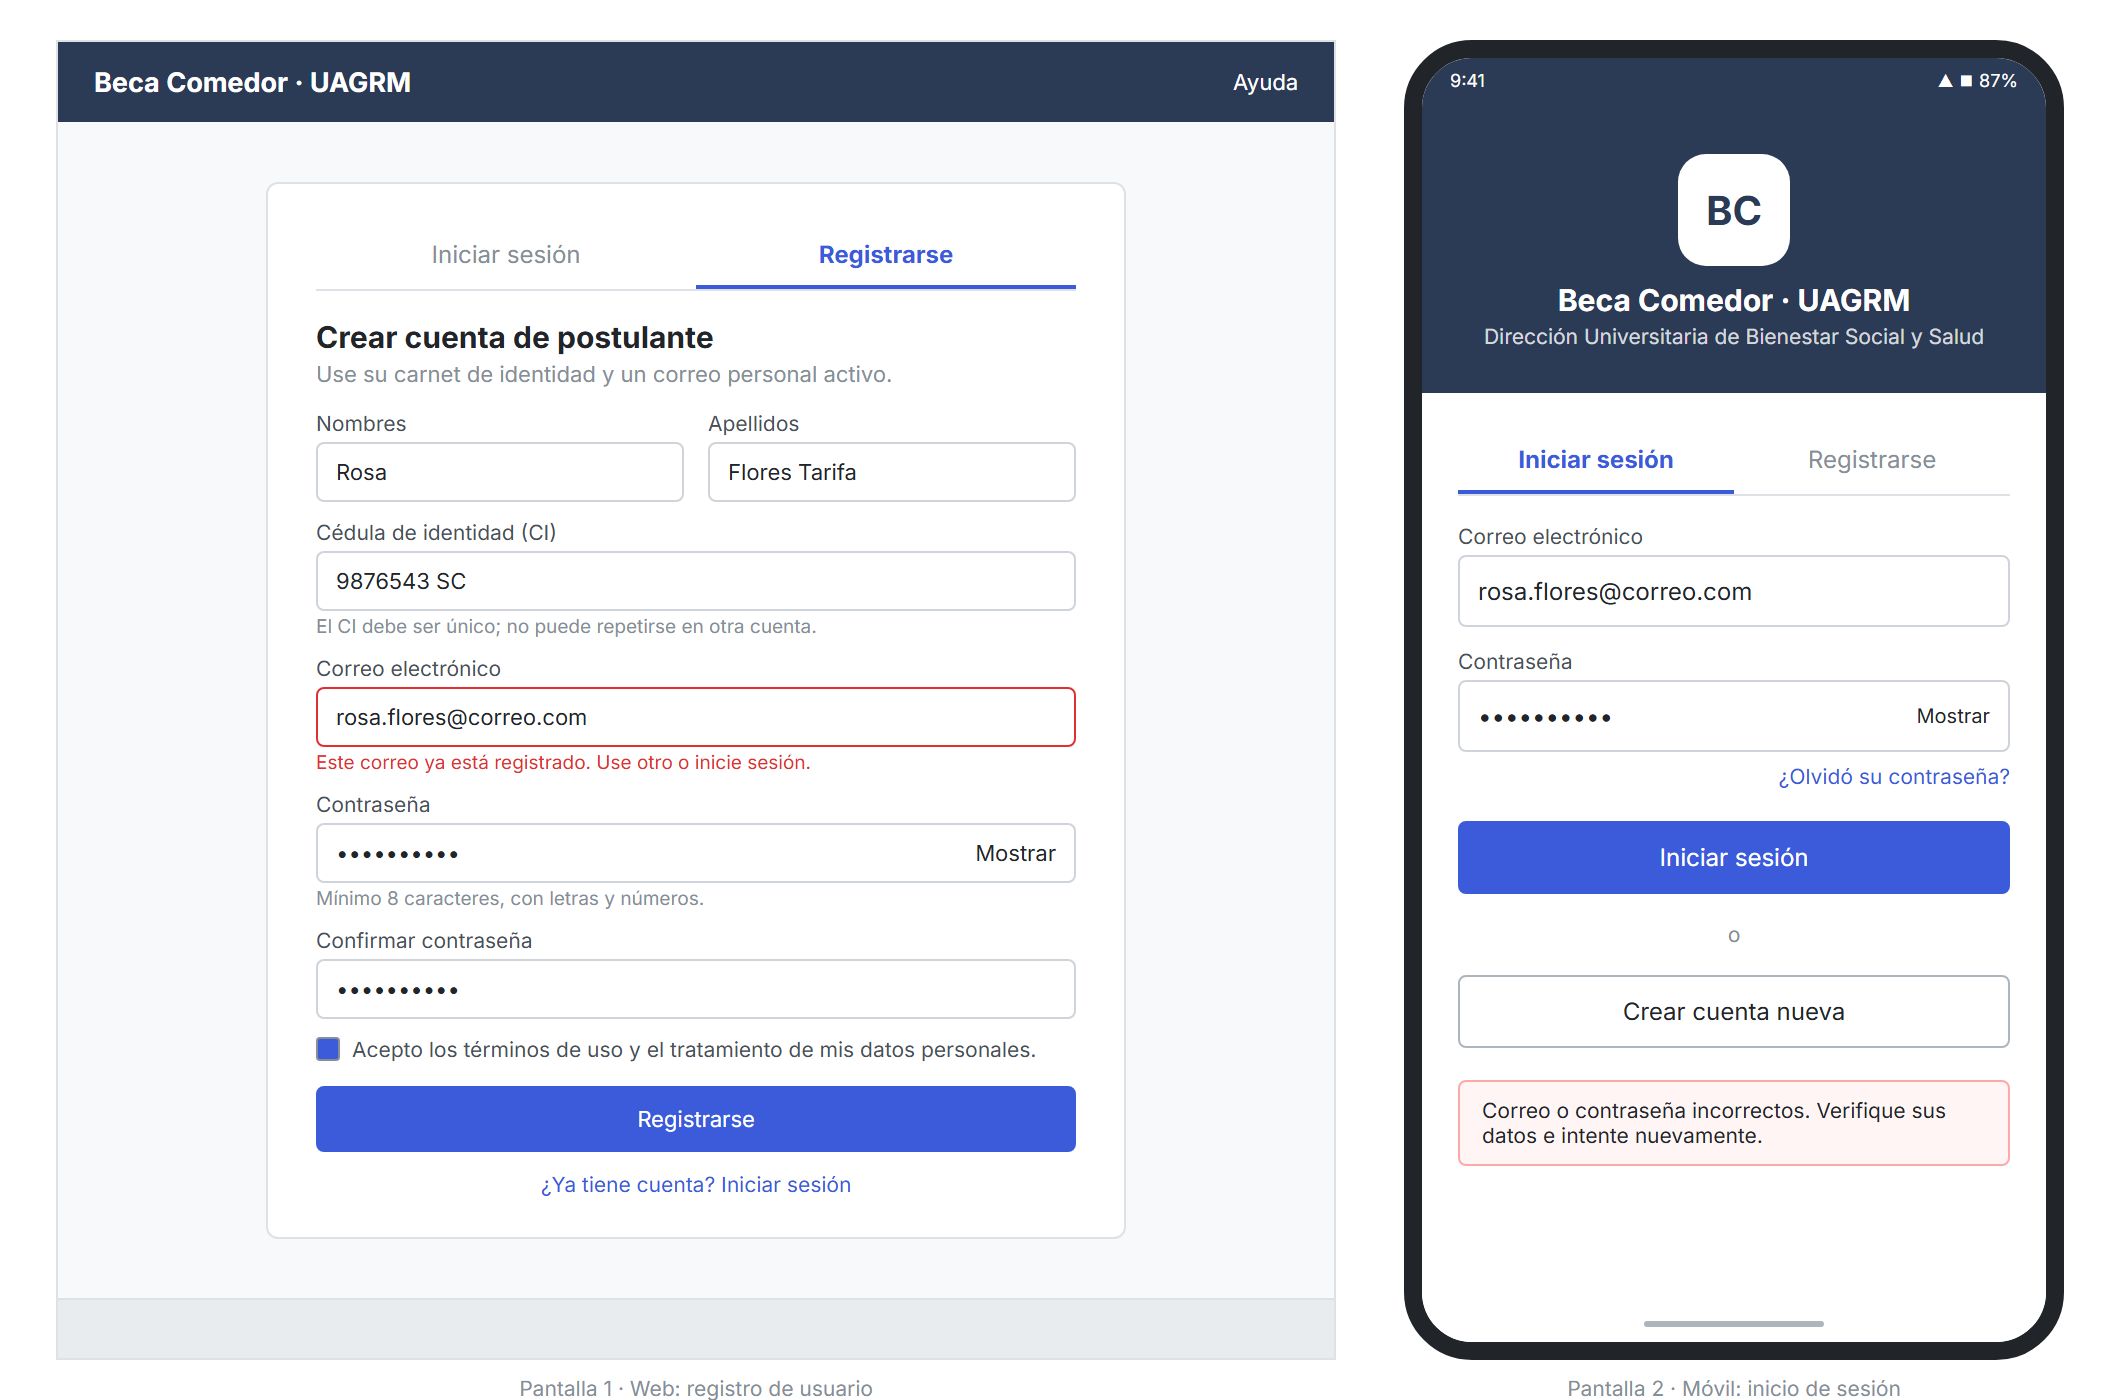
\includegraphics[width=\textwidth,height=0.75\textheight,keepaspectratio]{images/134_Mockup_CU01_Registrarse_autenticarse.png}

\smallskip
\noindent\raggedright\textit{Nota.} Elaboración propia.
\end{figure}



\Needspace{0.9\textheight}
\wfb{\wn{7}.5.2. Interfaz CU-02 Enviar postulación a Beca Comedor}\label{sec:cap7_interfaz_cu02}

La Figura~\ref{fig:mockup_cu02} presenta la maqueta de interfaz del CU-02.

\begin{figure}[H]
\caption{Maqueta de interfaz del CU-02 Enviar postulación a Beca Comedor}
\label{fig:mockup_cu02}
\centering
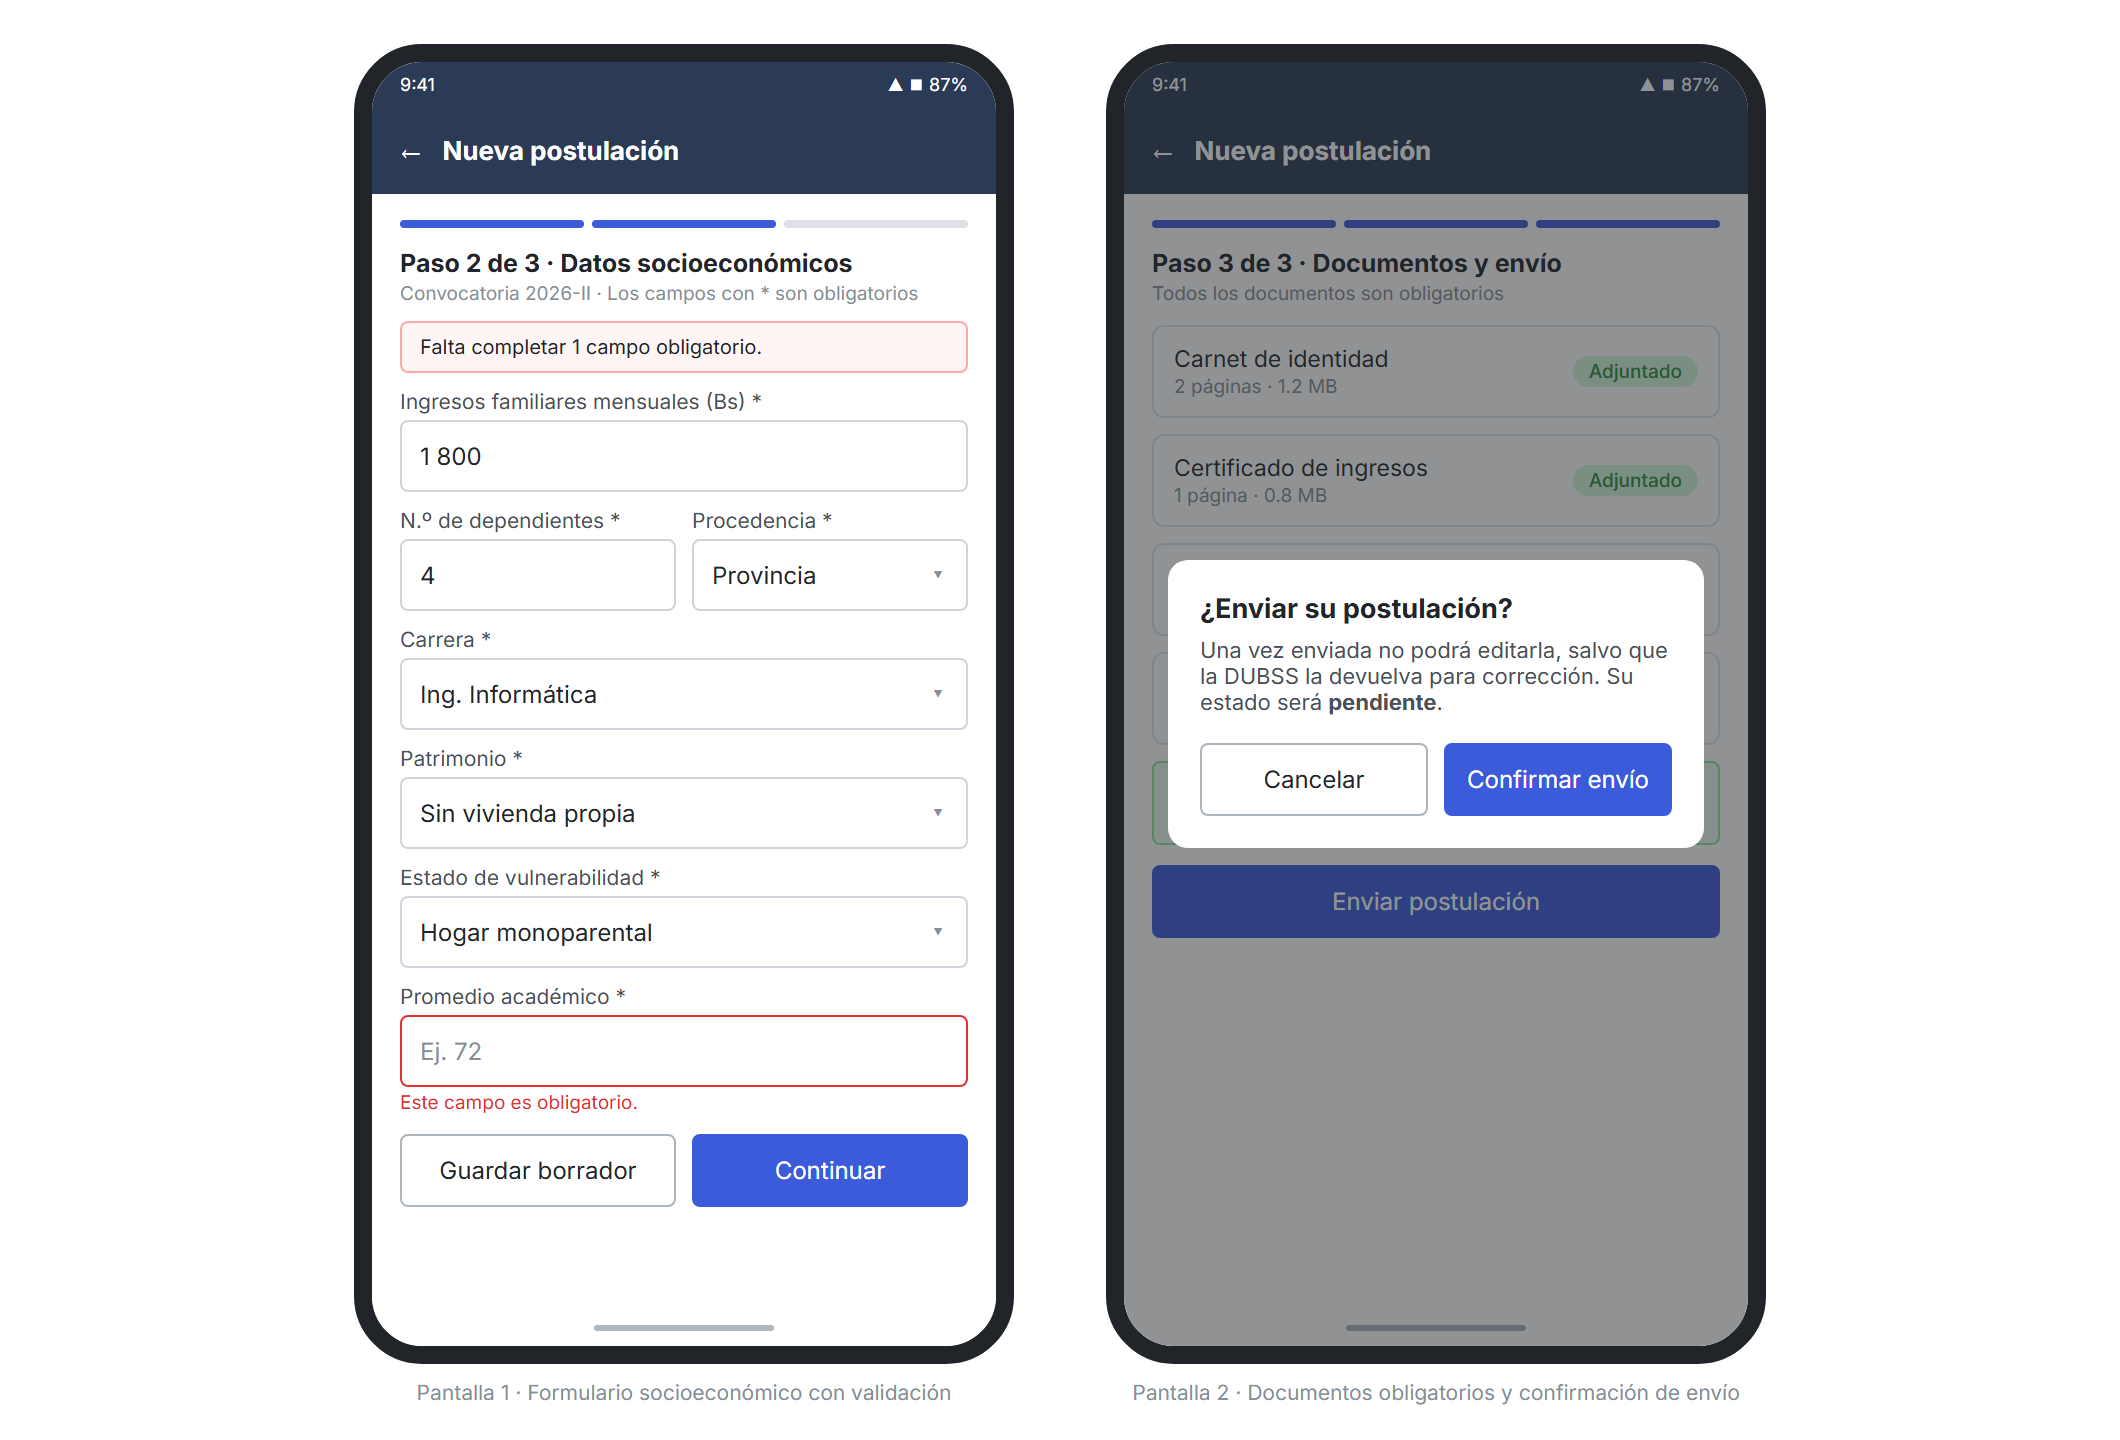
\includegraphics[width=\textwidth,height=0.75\textheight,keepaspectratio]{images/135_Mockup_CU02_Enviar_postulacion.png}

\smallskip
\noindent\raggedright\textit{Nota.} Elaboración propia.
\end{figure}



\Needspace{0.9\textheight}
\wfb{\wn{7}.5.3. Interfaz CU-03 Precalificar postulación con Inteligencia Artificial}\label{sec:cap7_interfaz_cu03}

La Figura~\ref{fig:mockup_cu03} presenta la maqueta de interfaz del CU-03.

\begin{figure}[H]
\caption{Maqueta de interfaz del CU-03 Precalificar postulación con Inteligencia Artificial}
\label{fig:mockup_cu03}
\centering
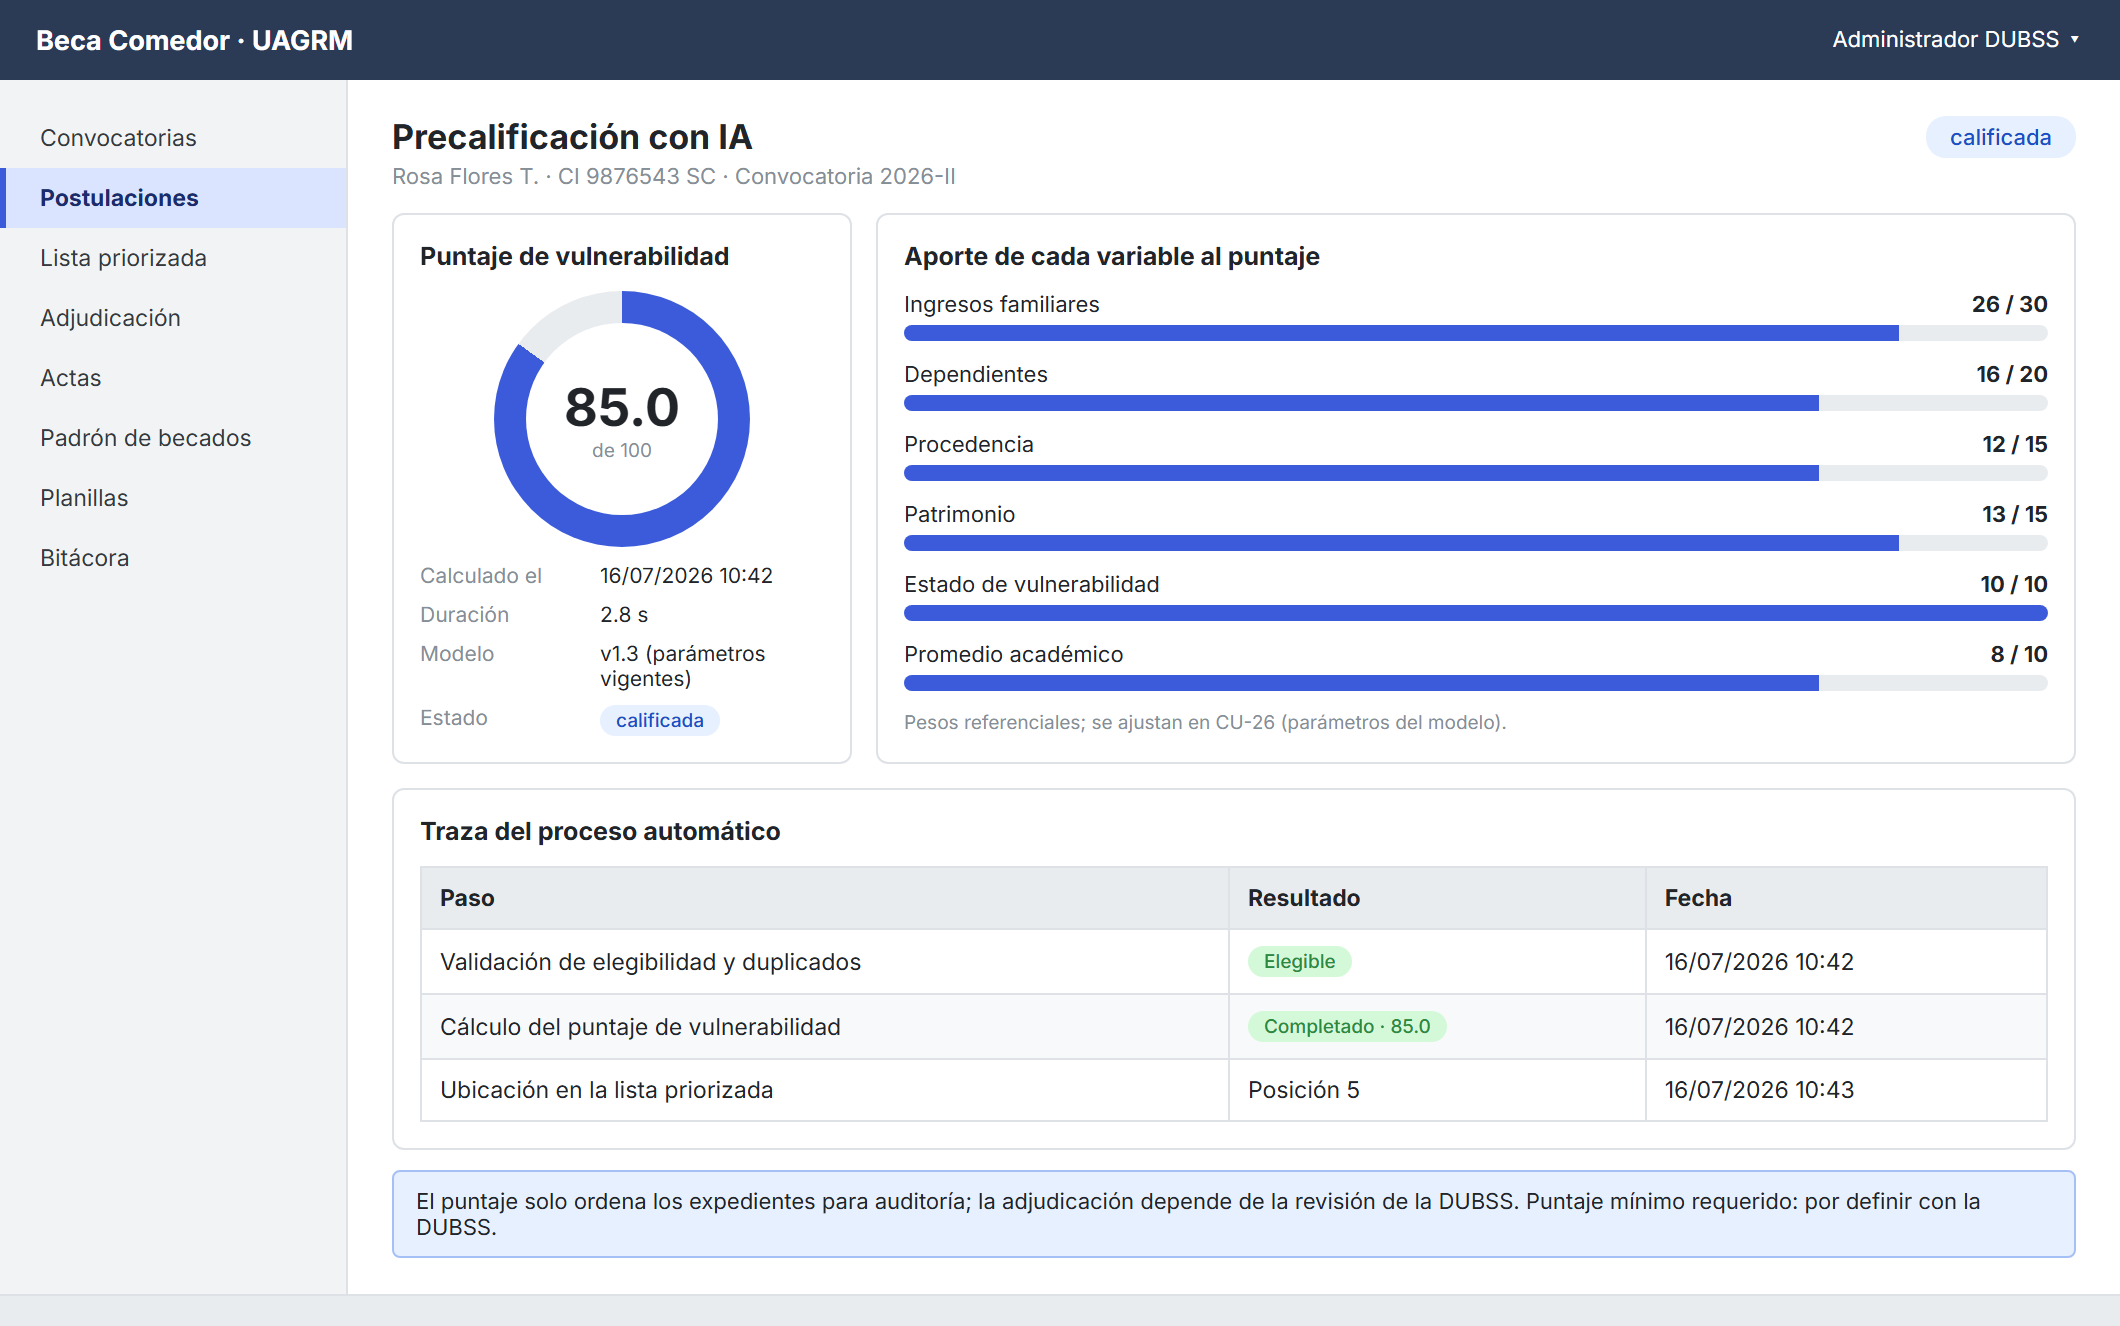
\includegraphics[width=\textwidth,height=0.75\textheight,keepaspectratio]{images/136_Mockup_CU03_Precalificar_IA.png}

\smallskip
\noindent\raggedright\textit{Nota.} Elaboración propia.
\end{figure}



\Needspace{0.9\textheight}
\wfb{\wn{7}.5.4. Interfaz CU-04 Consultar estado de postulación}\label{sec:cap7_interfaz_cu04}

La Figura~\ref{fig:mockup_cu04} presenta la maqueta de interfaz del CU-04.

\begin{figure}[H]
\caption{Maqueta de interfaz del CU-04 Consultar estado de postulación}
\label{fig:mockup_cu04}
\centering
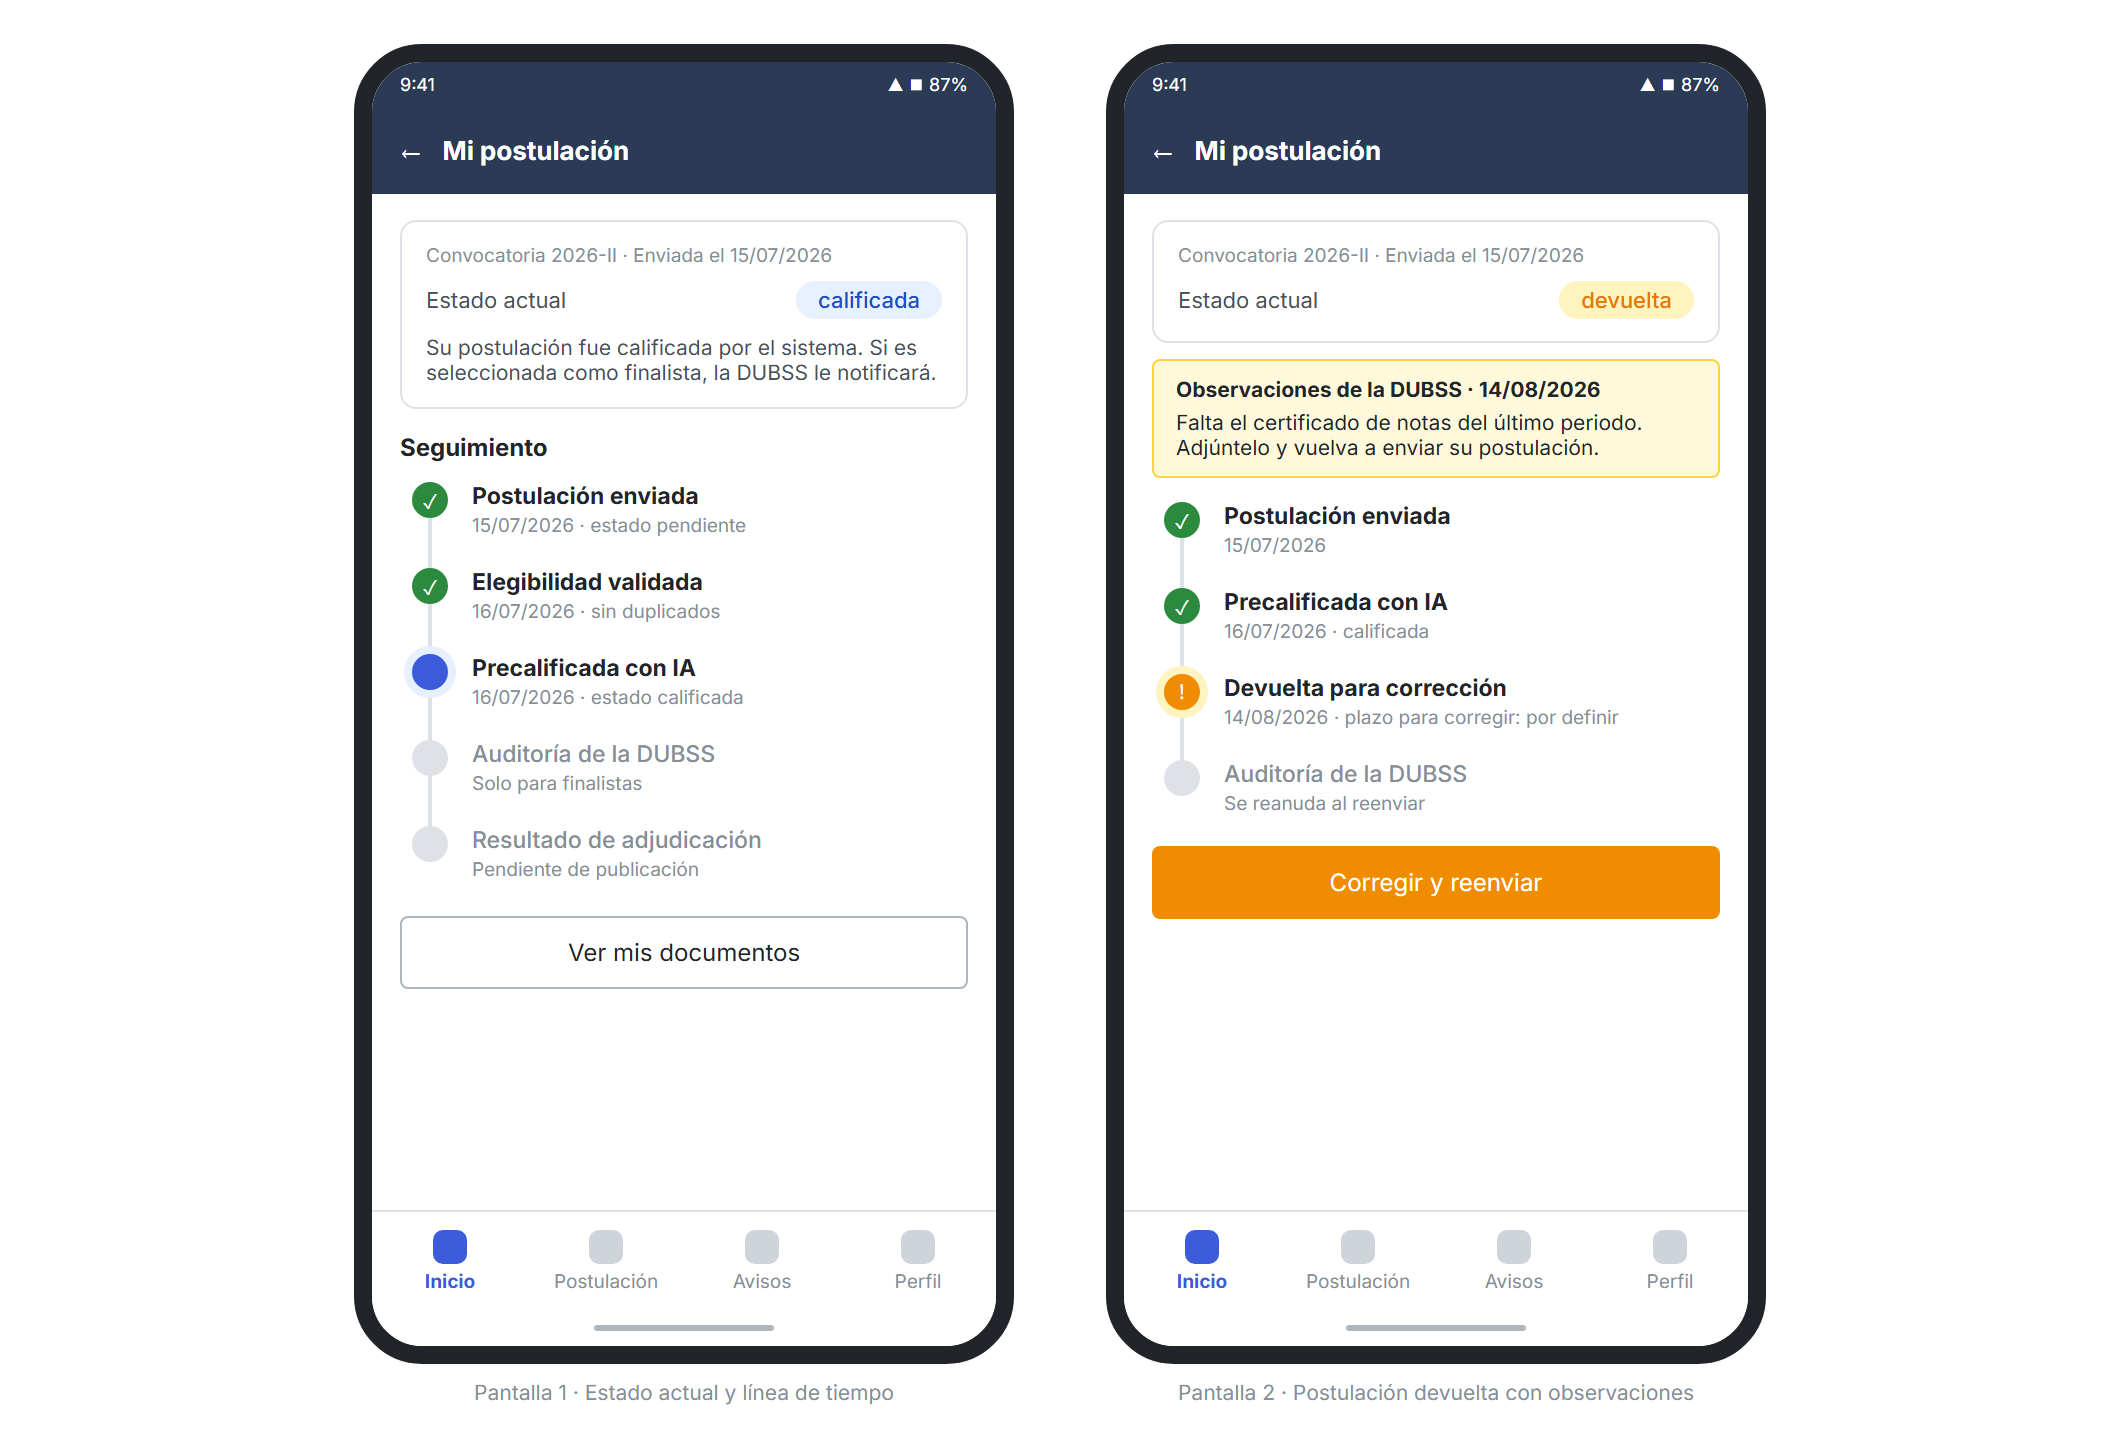
\includegraphics[width=\textwidth,height=0.75\textheight,keepaspectratio]{images/137_Mockup_CU04_Consultar_estado.png}

\smallskip
\noindent\raggedright\textit{Nota.} Elaboración propia.
\end{figure}



\Needspace{0.9\textheight}
\wfb{\wn{7}.5.5. Interfaz CU-05 Auditar y adjudicar becas}\label{sec:cap7_interfaz_cu05}

La Figura~\ref{fig:mockup_cu05} presenta la maqueta de interfaz del CU-05.

\begin{figure}[H]
\caption{Maqueta de interfaz del CU-05 Auditar y adjudicar becas}
\label{fig:mockup_cu05}
\centering
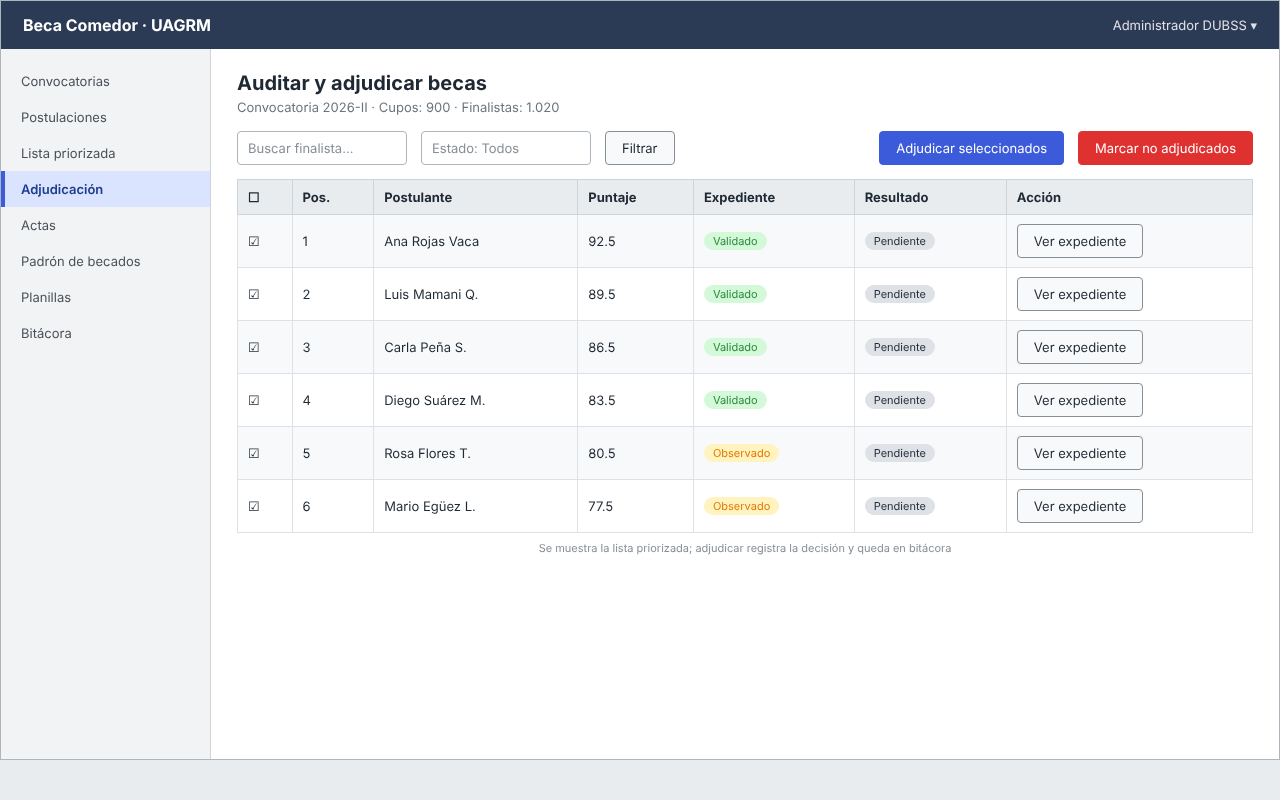
\includegraphics[width=\textwidth,height=0.75\textheight,keepaspectratio]{images/105_Mockup_CU05_Auditar_y_adjudicar_becas.png}

\smallskip
\noindent\raggedright\textit{Nota.} Elaboración propia.
\end{figure}


\Needspace{0.9\textheight}
\wfb{\wn{7}.5.6. Interfaz CU-06 Visualizar lista priorizada de postulantes}\label{sec:cap7_interfaz_cu06}

La Figura~\ref{fig:mockup_cu06} presenta la maqueta de interfaz del CU-06.

\begin{figure}[H]
\caption{Maqueta de interfaz del CU-06 Visualizar lista priorizada de postulantes}
\label{fig:mockup_cu06}
\centering
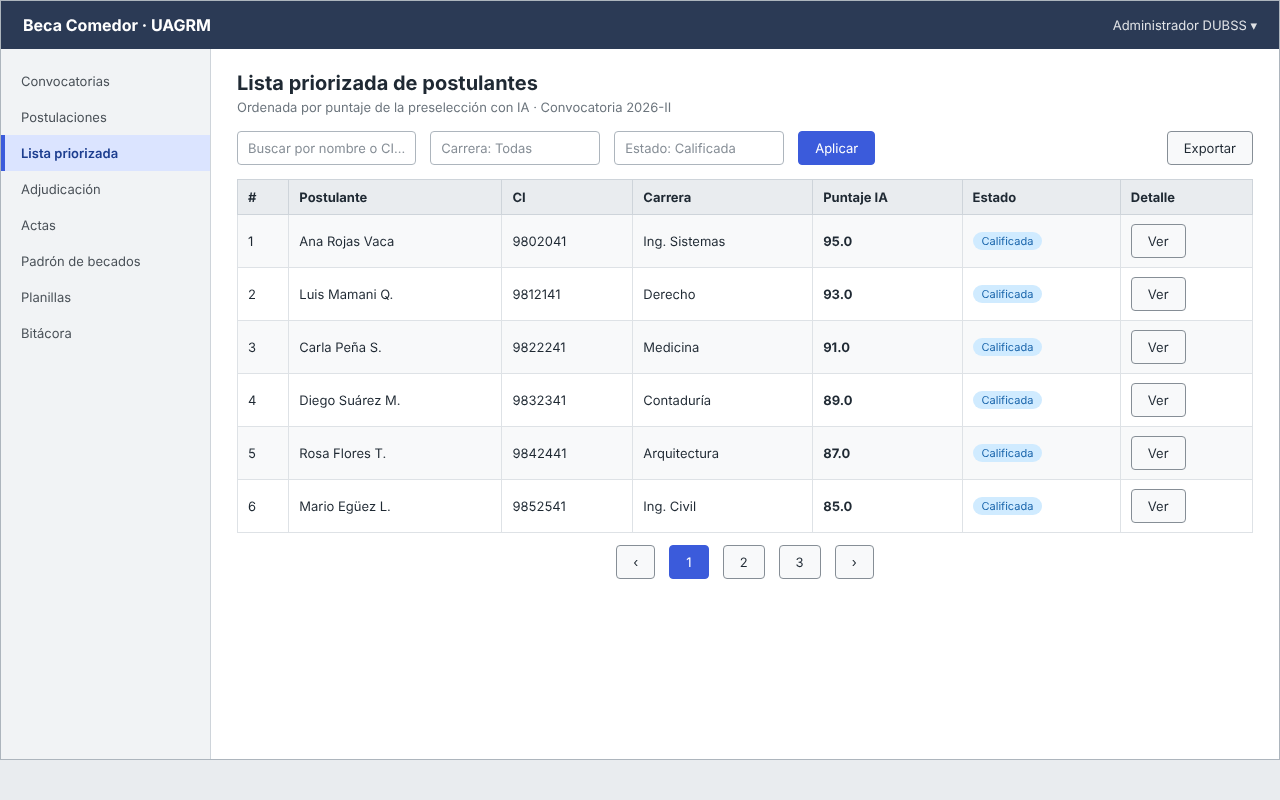
\includegraphics[width=\textwidth,height=0.75\textheight,keepaspectratio]{images/106_Mockup_CU06_Lista_priorizada.png}

\smallskip
\noindent\raggedright\textit{Nota.} Elaboración propia.
\end{figure}


\Needspace{0.9\textheight}
\wfb{\wn{7}.5.7. Interfaz CU-07 Auditar expediente finalista}\label{sec:cap7_interfaz_cu07}

La Figura~\ref{fig:mockup_cu07} presenta la maqueta de interfaz del CU-07.

\begin{figure}[H]
\caption{Maqueta de interfaz del CU-07 Auditar expediente finalista}
\label{fig:mockup_cu07}
\centering
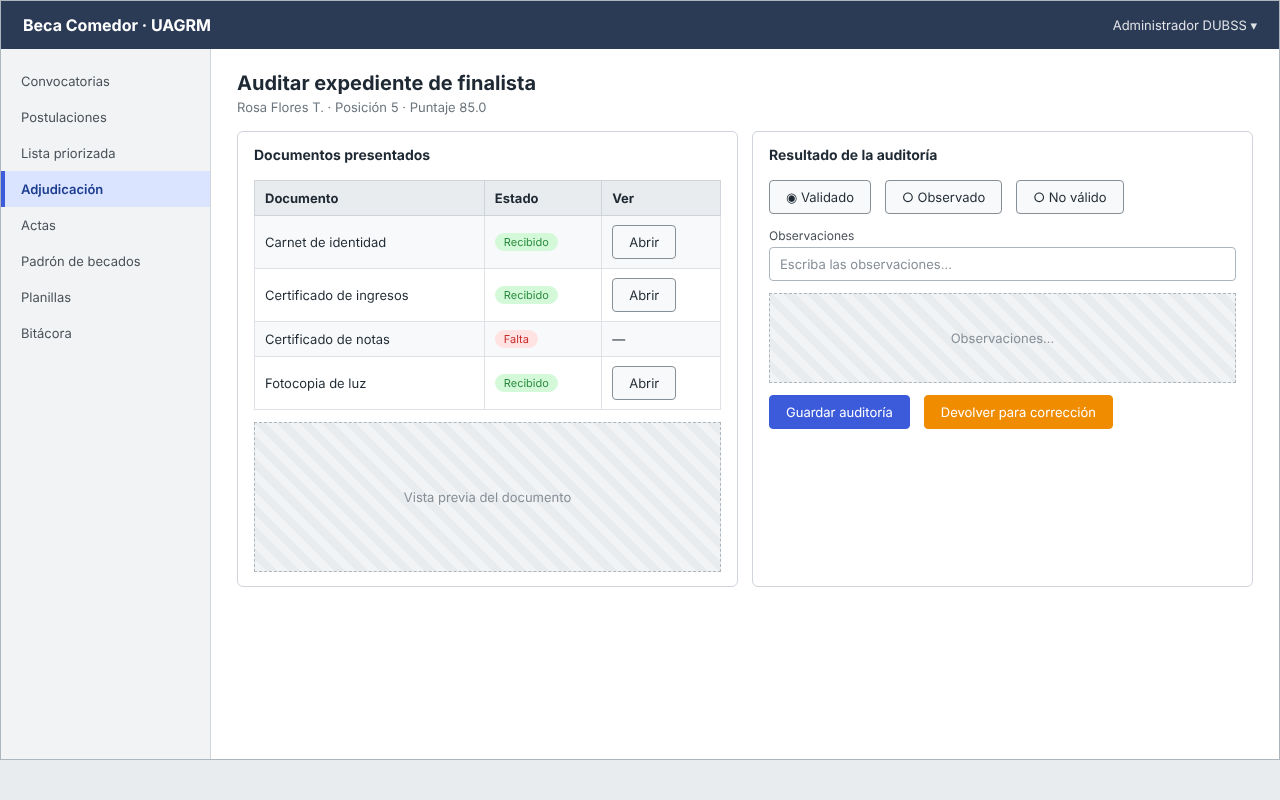
\includegraphics[width=\textwidth,height=0.75\textheight,keepaspectratio]{images/107_Mockup_CU07_Auditar_expediente_finalista.png}

\smallskip
\noindent\raggedright\textit{Nota.} Elaboración propia.
\end{figure}


\Needspace{0.9\textheight}
\wfb{\wn{7}.5.8. Interfaz CU-08 Generar acta de adjudicación}\label{sec:cap7_interfaz_cu08}

La Figura~\ref{fig:mockup_cu08} presenta la maqueta de interfaz del CU-08.

\begin{figure}[H]
\caption{Maqueta de interfaz del CU-08 Generar acta de adjudicación}
\label{fig:mockup_cu08}
\centering
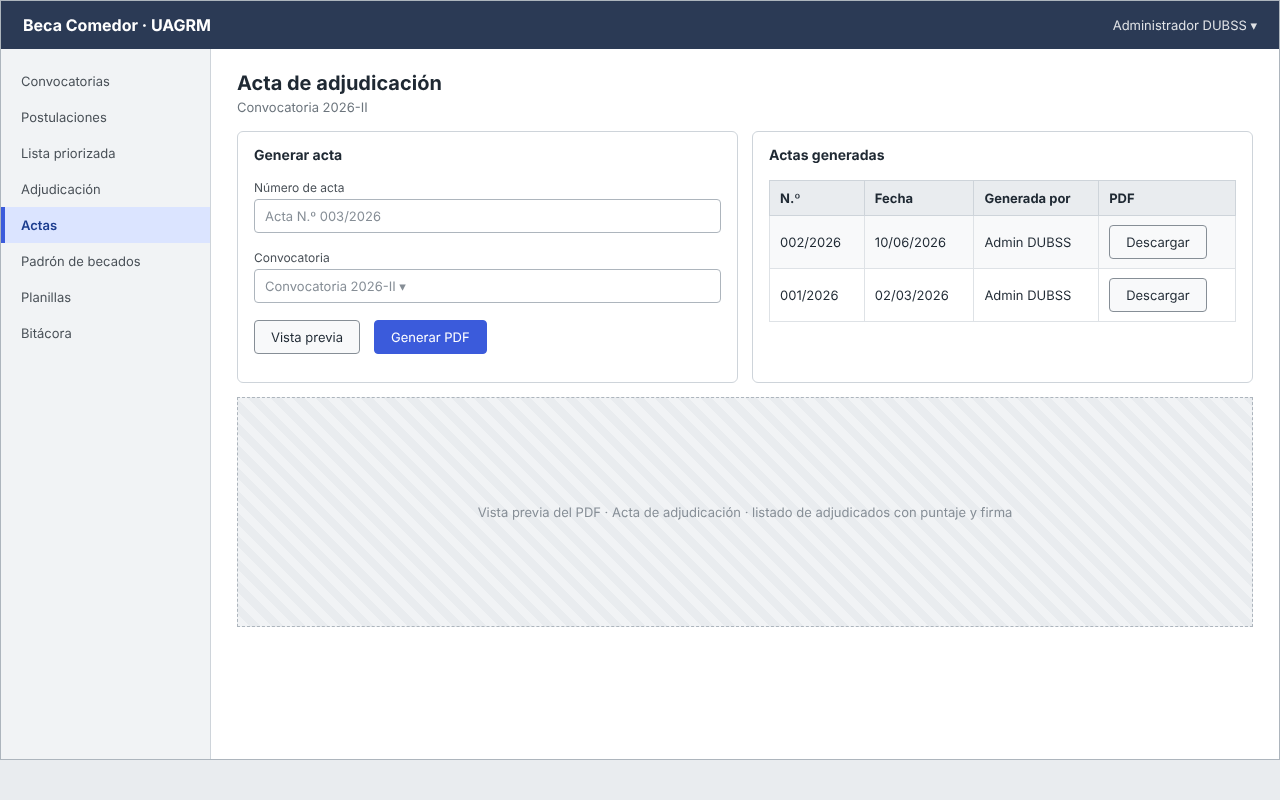
\includegraphics[width=\textwidth,height=0.75\textheight,keepaspectratio]{images/108_Mockup_CU08_Acta_de_adjudicacion.png}

\smallskip
\noindent\raggedright\textit{Nota.} Elaboración propia.
\end{figure}


\Needspace{0.9\textheight}
\wfb{\wn{7}.5.9. Interfaz CU-09 Generar planilla de asistencia}\label{sec:cap7_interfaz_cu09}

La Figura~\ref{fig:mockup_cu09} presenta la maqueta de interfaz del CU-09.

\begin{figure}[H]
\caption{Maqueta de interfaz del CU-09 Generar planilla de asistencia}
\label{fig:mockup_cu09}
\centering
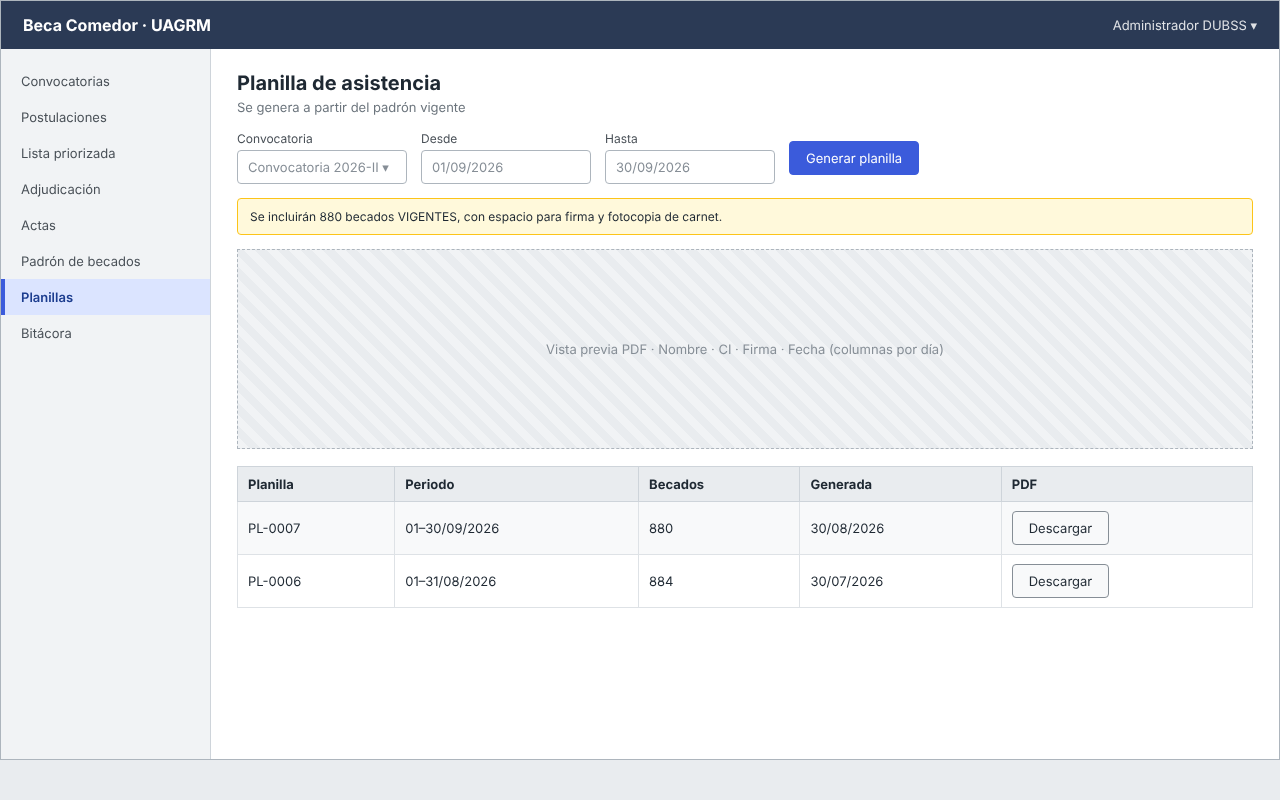
\includegraphics[width=\textwidth,height=0.75\textheight,keepaspectratio]{images/109_Mockup_CU09_Planilla_de_asistencia.png}

\smallskip
\noindent\raggedright\textit{Nota.} Elaboración propia.
\end{figure}


\Needspace{0.9\textheight}
\wfb{\wn{7}.5.10. Interfaz CU-10 Registrar asistencia digital}\label{sec:cap7_interfaz_cu10}

La Figura~\ref{fig:mockup_cu10} presenta la maqueta de interfaz del CU-10.

\begin{figure}[H]
\caption{Maqueta de interfaz del CU-10 Registrar asistencia digital}
\label{fig:mockup_cu10}
\centering
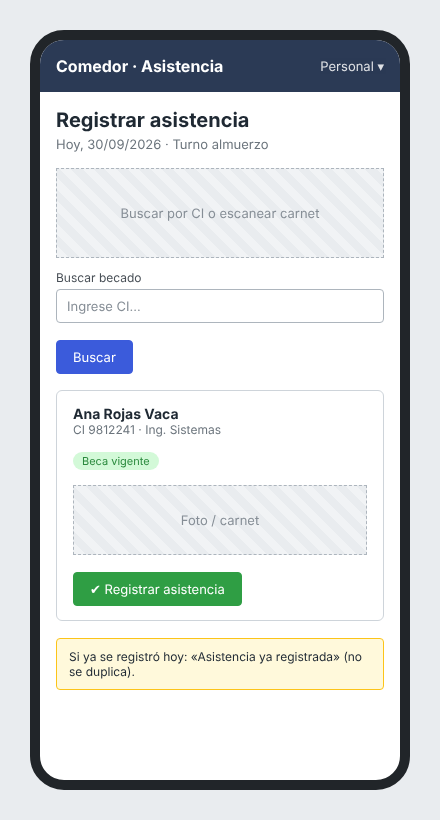
\includegraphics[width=\textwidth,height=0.75\textheight,keepaspectratio]{images/110_Mockup_CU10_Registrar_asistencia_digital.png}

\smallskip
\noindent\raggedright\textit{Nota.} Elaboración propia.
\end{figure}


\Needspace{0.9\textheight}
\wfb{\wn{7}.5.11. Interfaz CU-11 Cotejar registro contra respaldo físico}\label{sec:cap7_interfaz_cu11}

La Figura~\ref{fig:mockup_cu11} presenta la maqueta de interfaz del CU-11.

\begin{figure}[H]
\caption{Maqueta de interfaz del CU-11 Cotejar registro contra respaldo físico}
\label{fig:mockup_cu11}
\centering
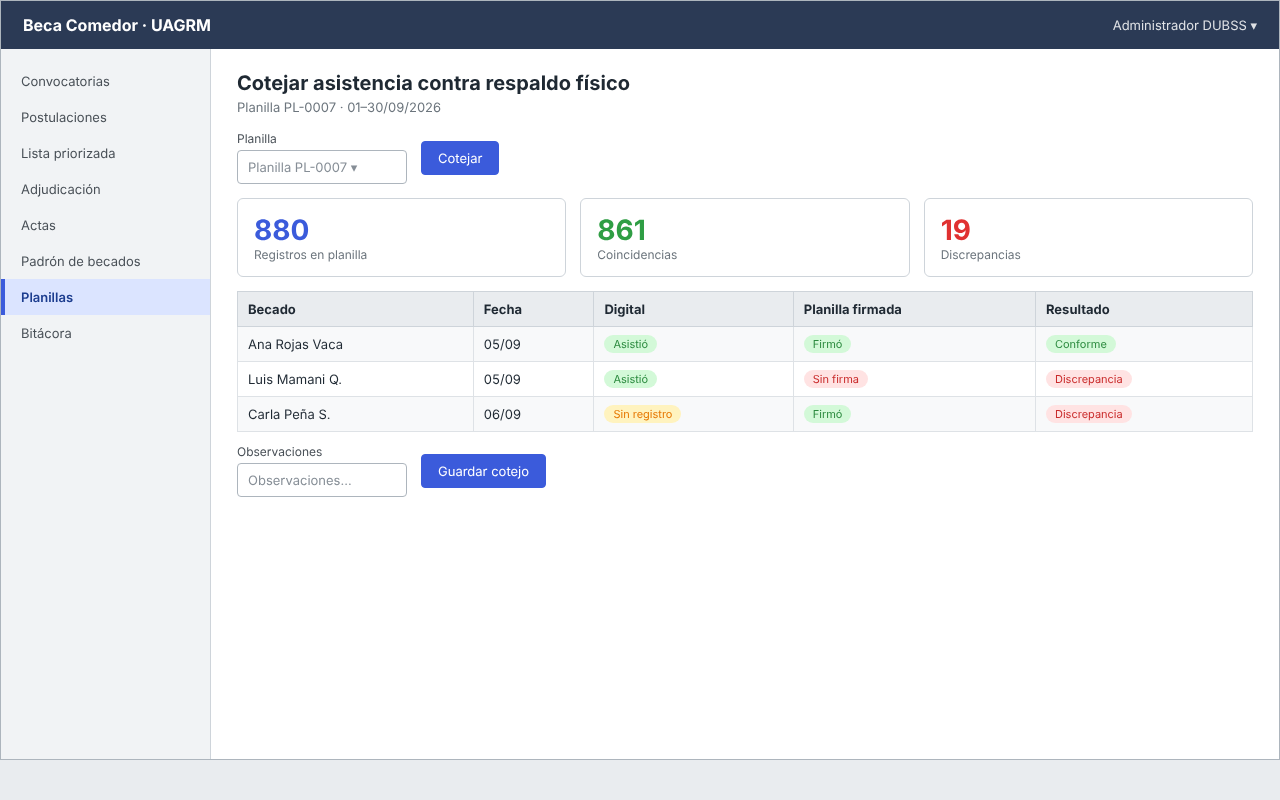
\includegraphics[width=\textwidth,height=0.75\textheight,keepaspectratio]{images/111_Mockup_CU11_Cotejar_contra_respaldo_fisico.png}

\smallskip
\noindent\raggedright\textit{Nota.} Elaboración propia.
\end{figure}


\Needspace{0.9\textheight}
\wfb{\wn{7}.5.12. Interfaz CU-12 Visualizar dashboard de indicadores BI}\label{sec:cap7_interfaz_cu12}

La Figura~\ref{fig:mockup_cu12} presenta la maqueta de interfaz del CU-12.

\begin{figure}[H]
\caption{Maqueta de interfaz del CU-12 Visualizar dashboard de indicadores BI}
\label{fig:mockup_cu12}
\centering
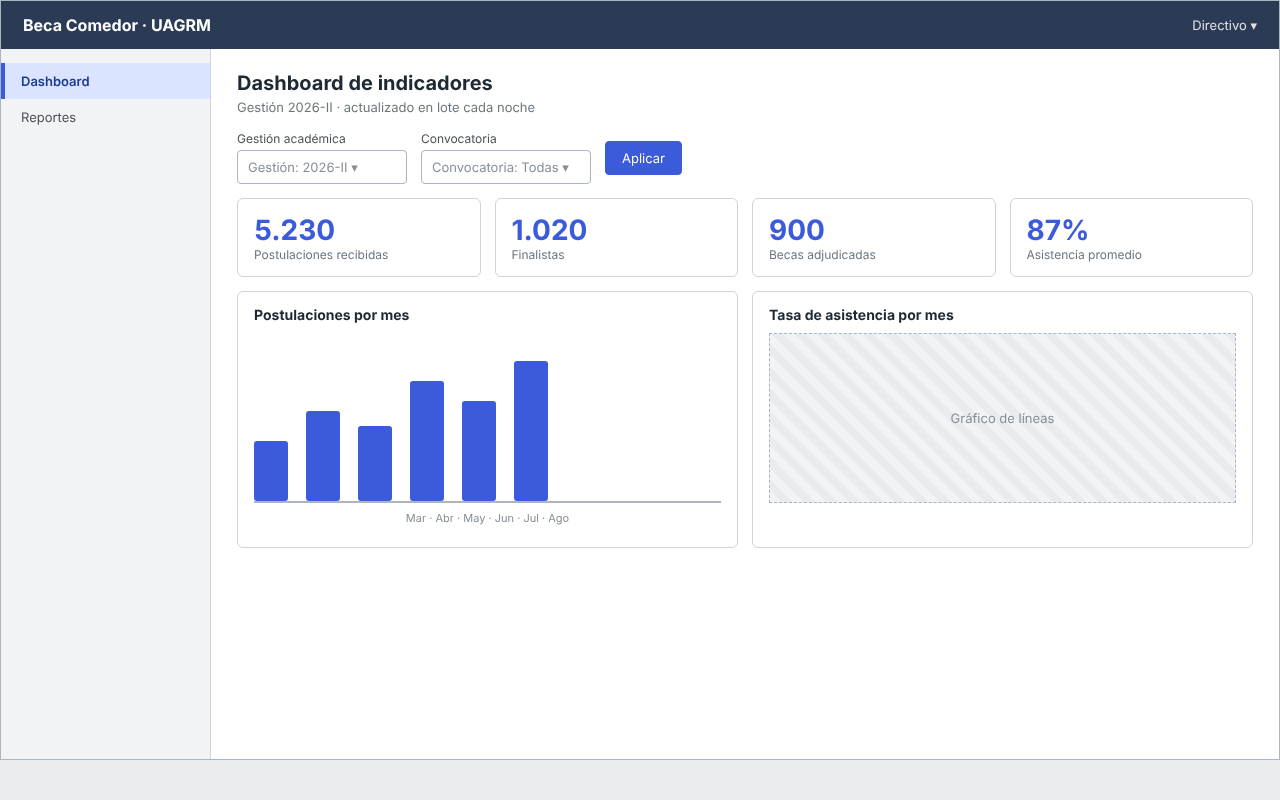
\includegraphics[width=\textwidth,height=0.75\textheight,keepaspectratio]{images/112_Mockup_CU12_Dashboard_BI.png}

\smallskip
\noindent\raggedright\textit{Nota.} Elaboración propia.
\end{figure}


\Needspace{0.9\textheight}
\wfb{\wn{7}.5.13. Interfaz CU-13 Gestionar convocatoria y gestión académica}\label{sec:cap7_interfaz_cu13}

La Figura~\ref{fig:mockup_cu13} presenta la maqueta de interfaz del CU-13.

\begin{figure}[H]
\caption{Maqueta de interfaz del CU-13 Gestionar convocatoria y gestión académica}
\label{fig:mockup_cu13}
\centering
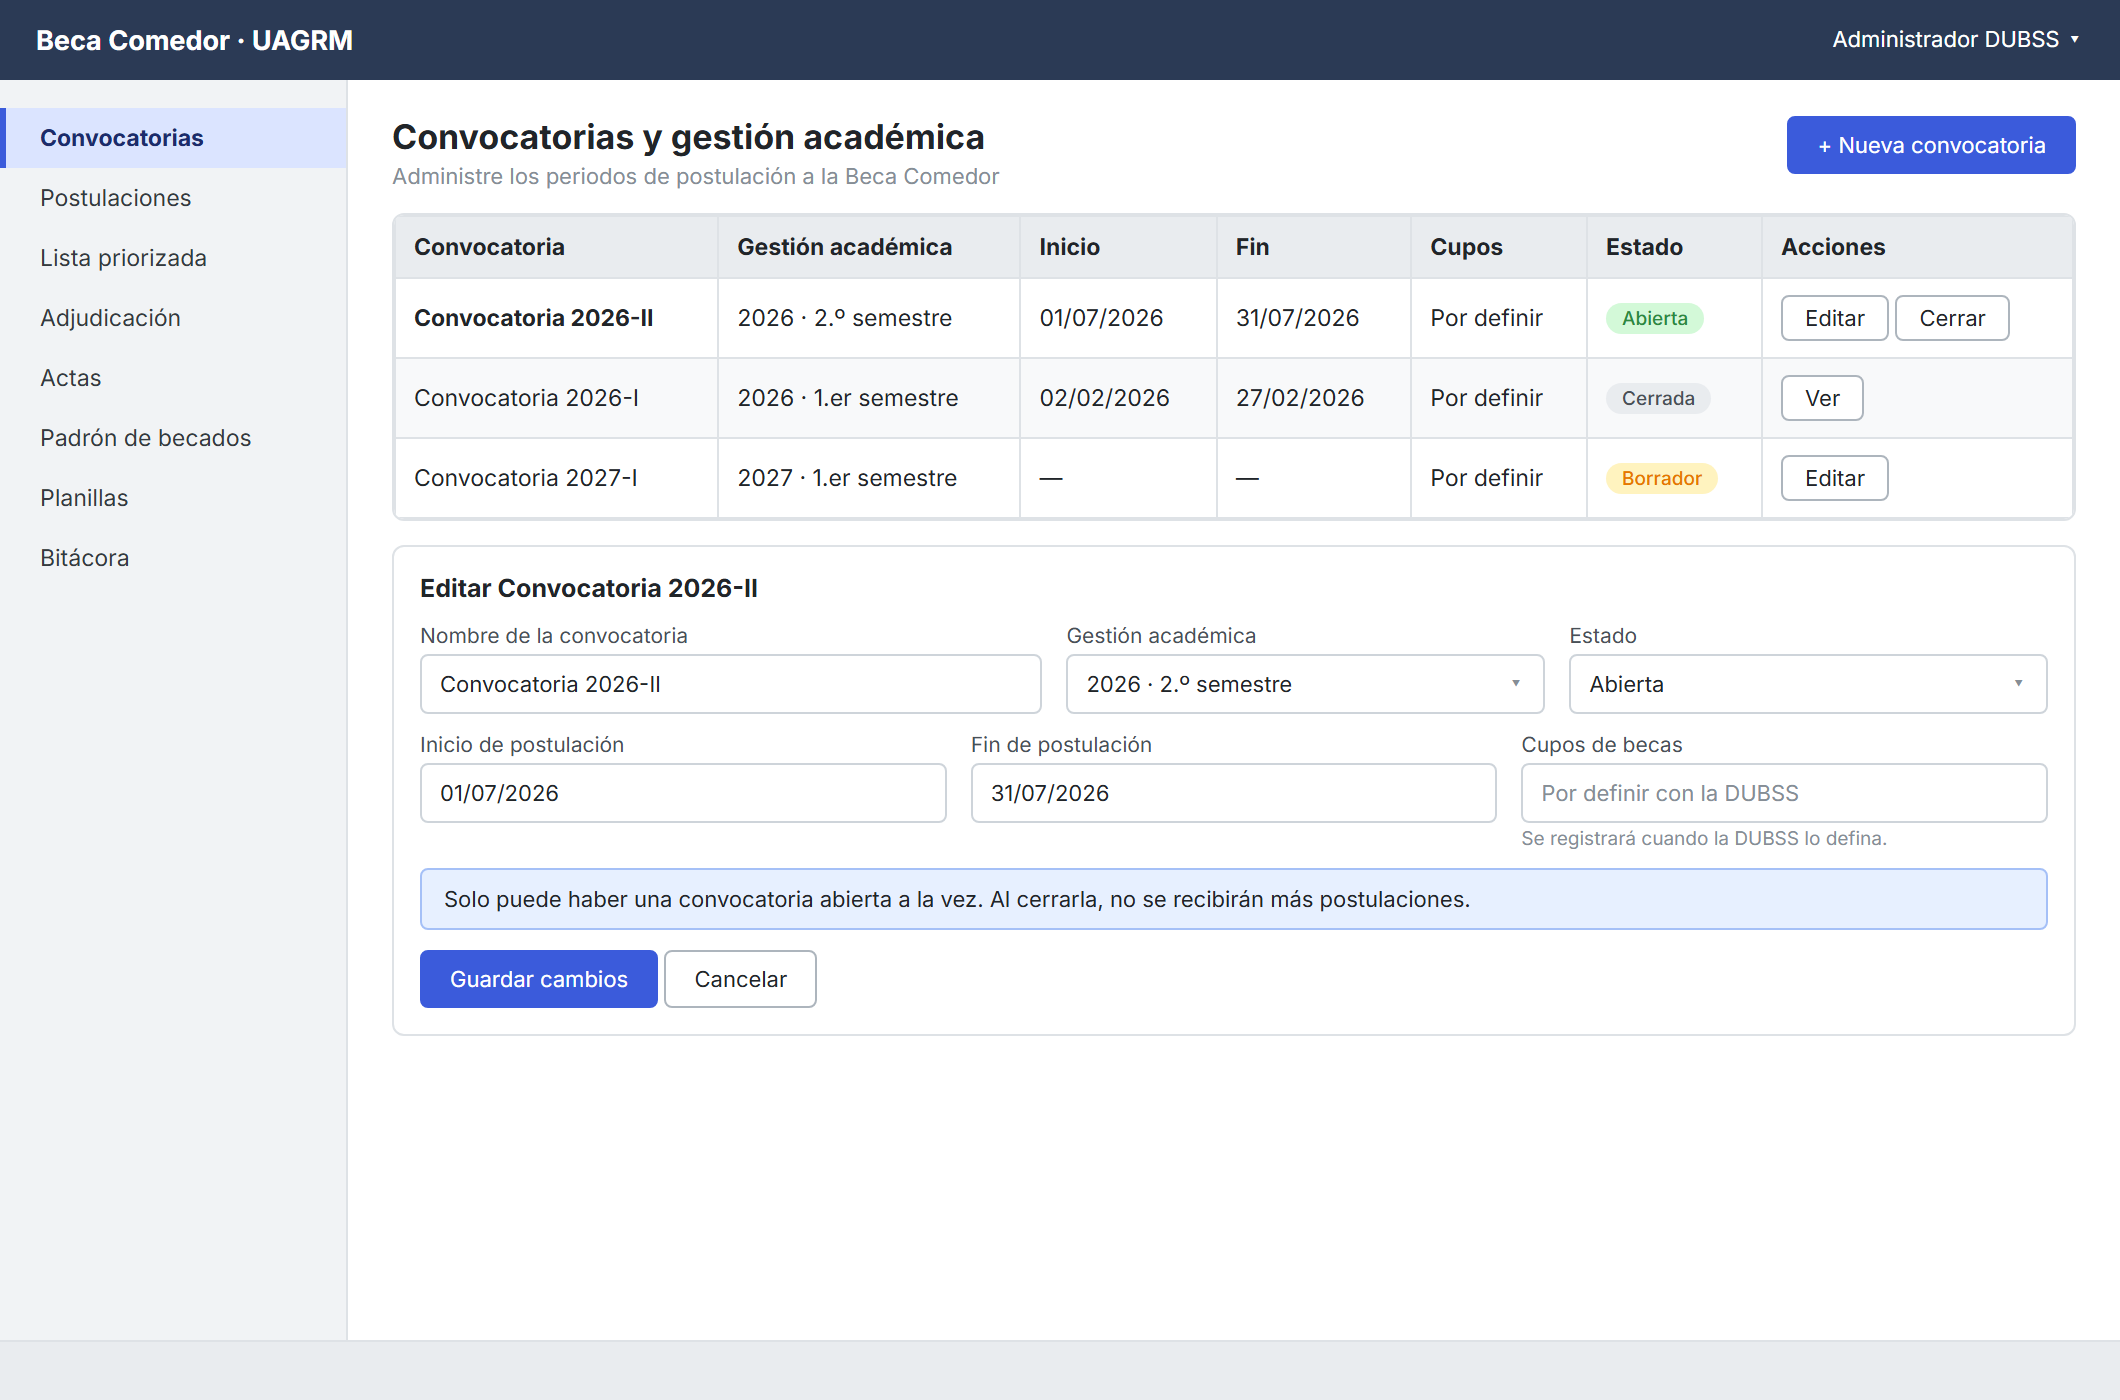
\includegraphics[width=\textwidth,height=0.75\textheight,keepaspectratio]{images/138_Mockup_CU13_Gestionar_convocatoria.png}

\smallskip
\noindent\raggedright\textit{Nota.} Elaboración propia.
\end{figure}



\Needspace{0.9\textheight}
\wfb{\wn{7}.5.14. Interfaz CU-14 Gestionar usuarios y roles}\label{sec:cap7_interfaz_cu14}

La Figura~\ref{fig:mockup_cu14} presenta la maqueta de interfaz del CU-14.

\begin{figure}[H]
\caption{Maqueta de interfaz del CU-14 Gestionar usuarios y roles}
\label{fig:mockup_cu14}
\centering
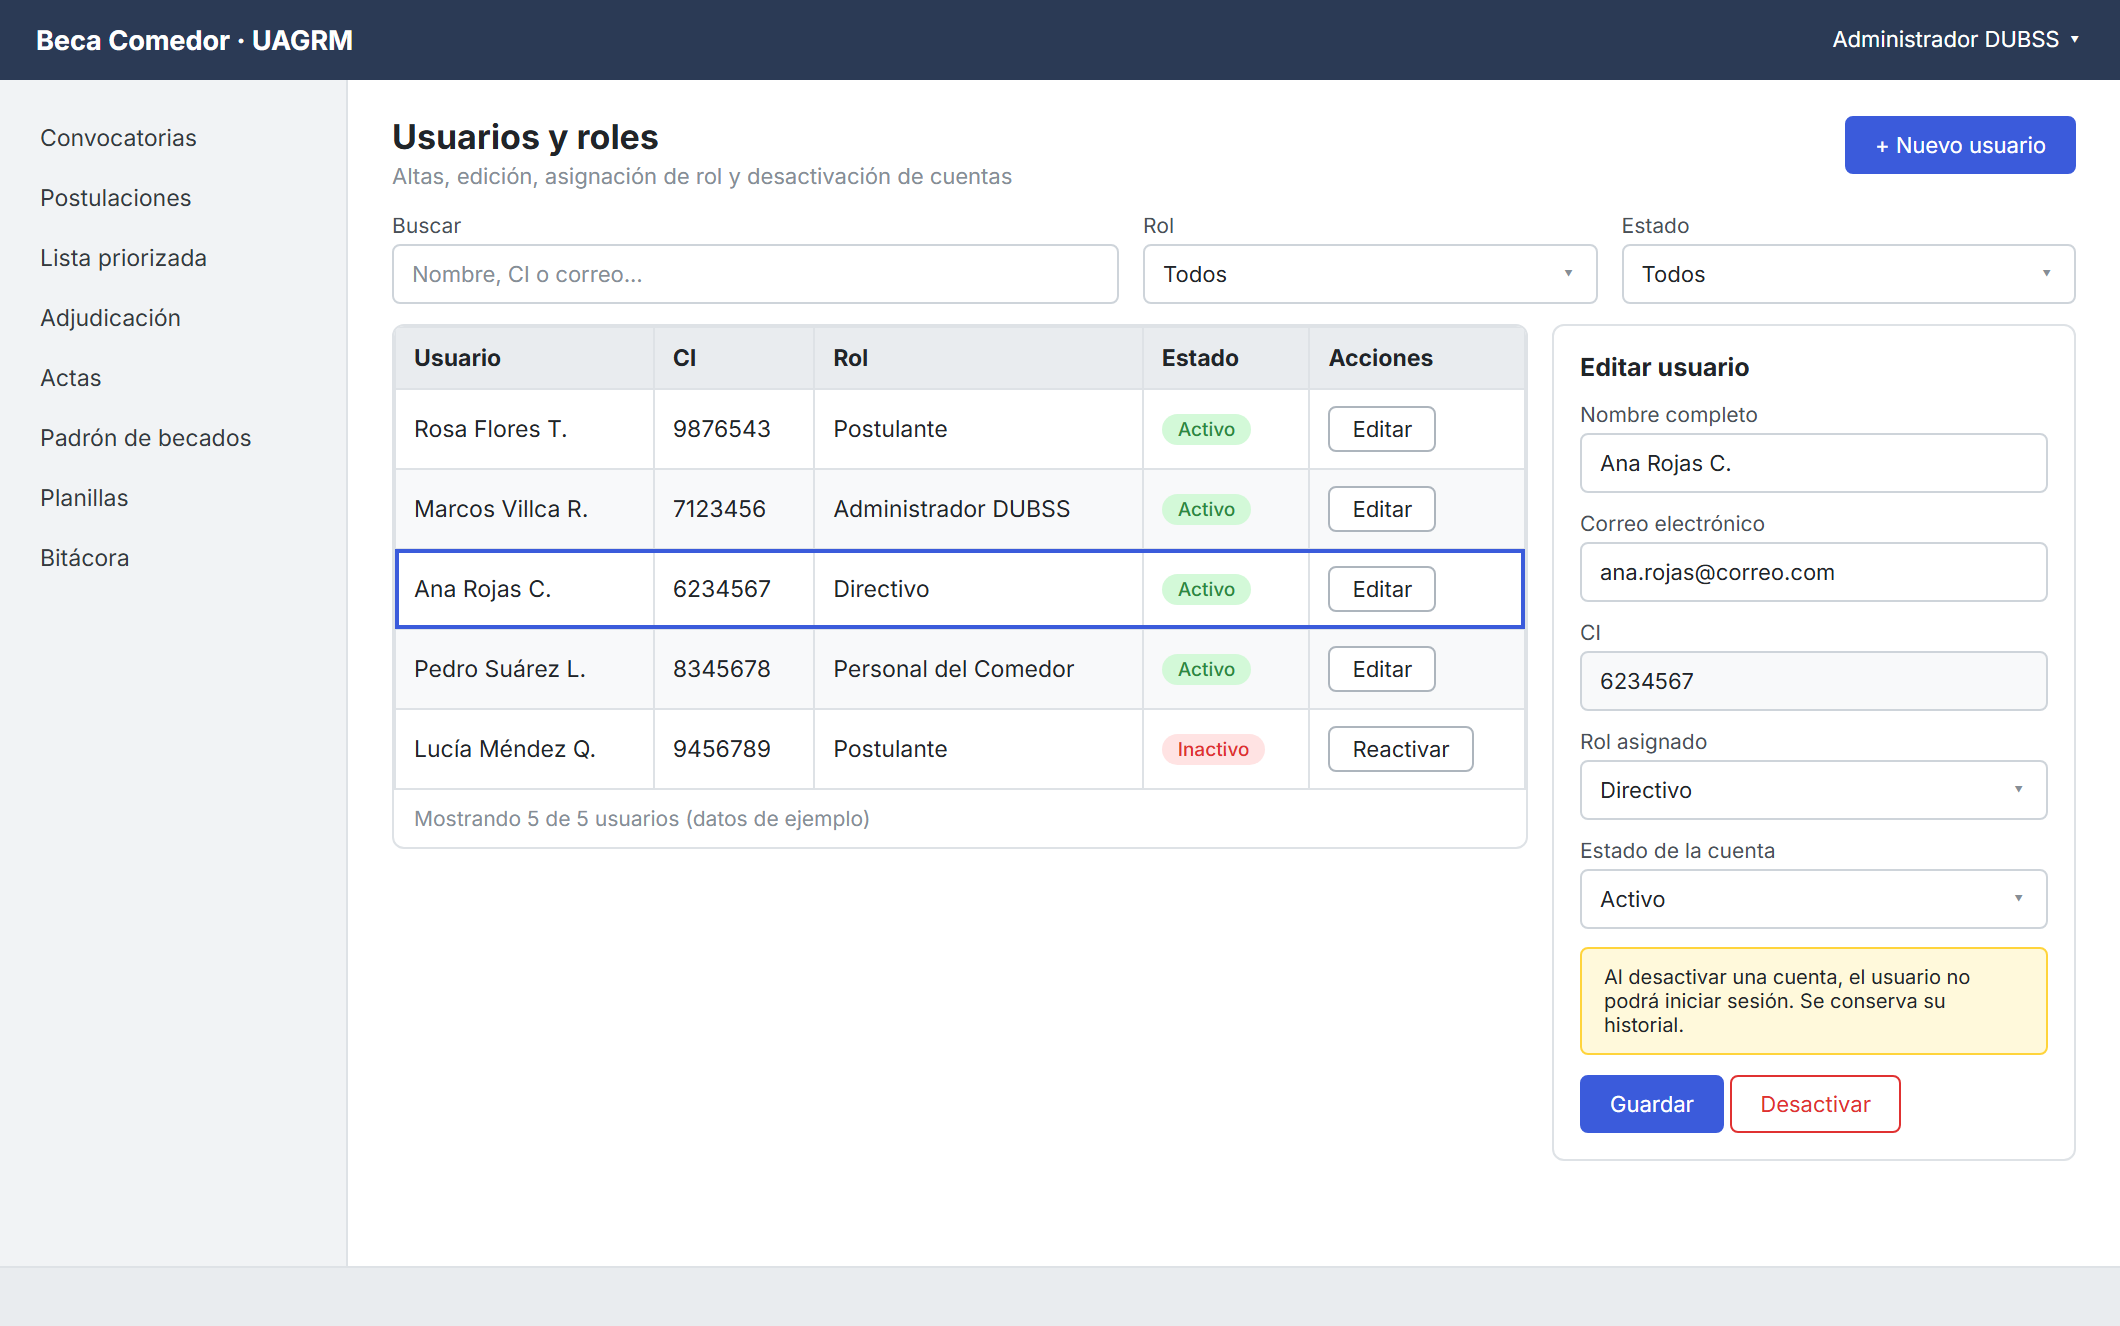
\includegraphics[width=\textwidth,height=0.75\textheight,keepaspectratio]{images/139_Mockup_CU14_Gestionar_usuarios_roles.png}

\smallskip
\noindent\raggedright\textit{Nota.} Elaboración propia.
\end{figure}



\Needspace{0.9\textheight}
\wfb{\wn{7}.5.15. Interfaz CU-15 Recuperar contraseña / gestionar perfil}\label{sec:cap7_interfaz_cu15}

La Figura~\ref{fig:mockup_cu15} presenta la maqueta de interfaz del CU-15.

\begin{figure}[H]
\caption{Maqueta de interfaz del CU-15 Recuperar contraseña / gestionar perfil}
\label{fig:mockup_cu15}
\centering
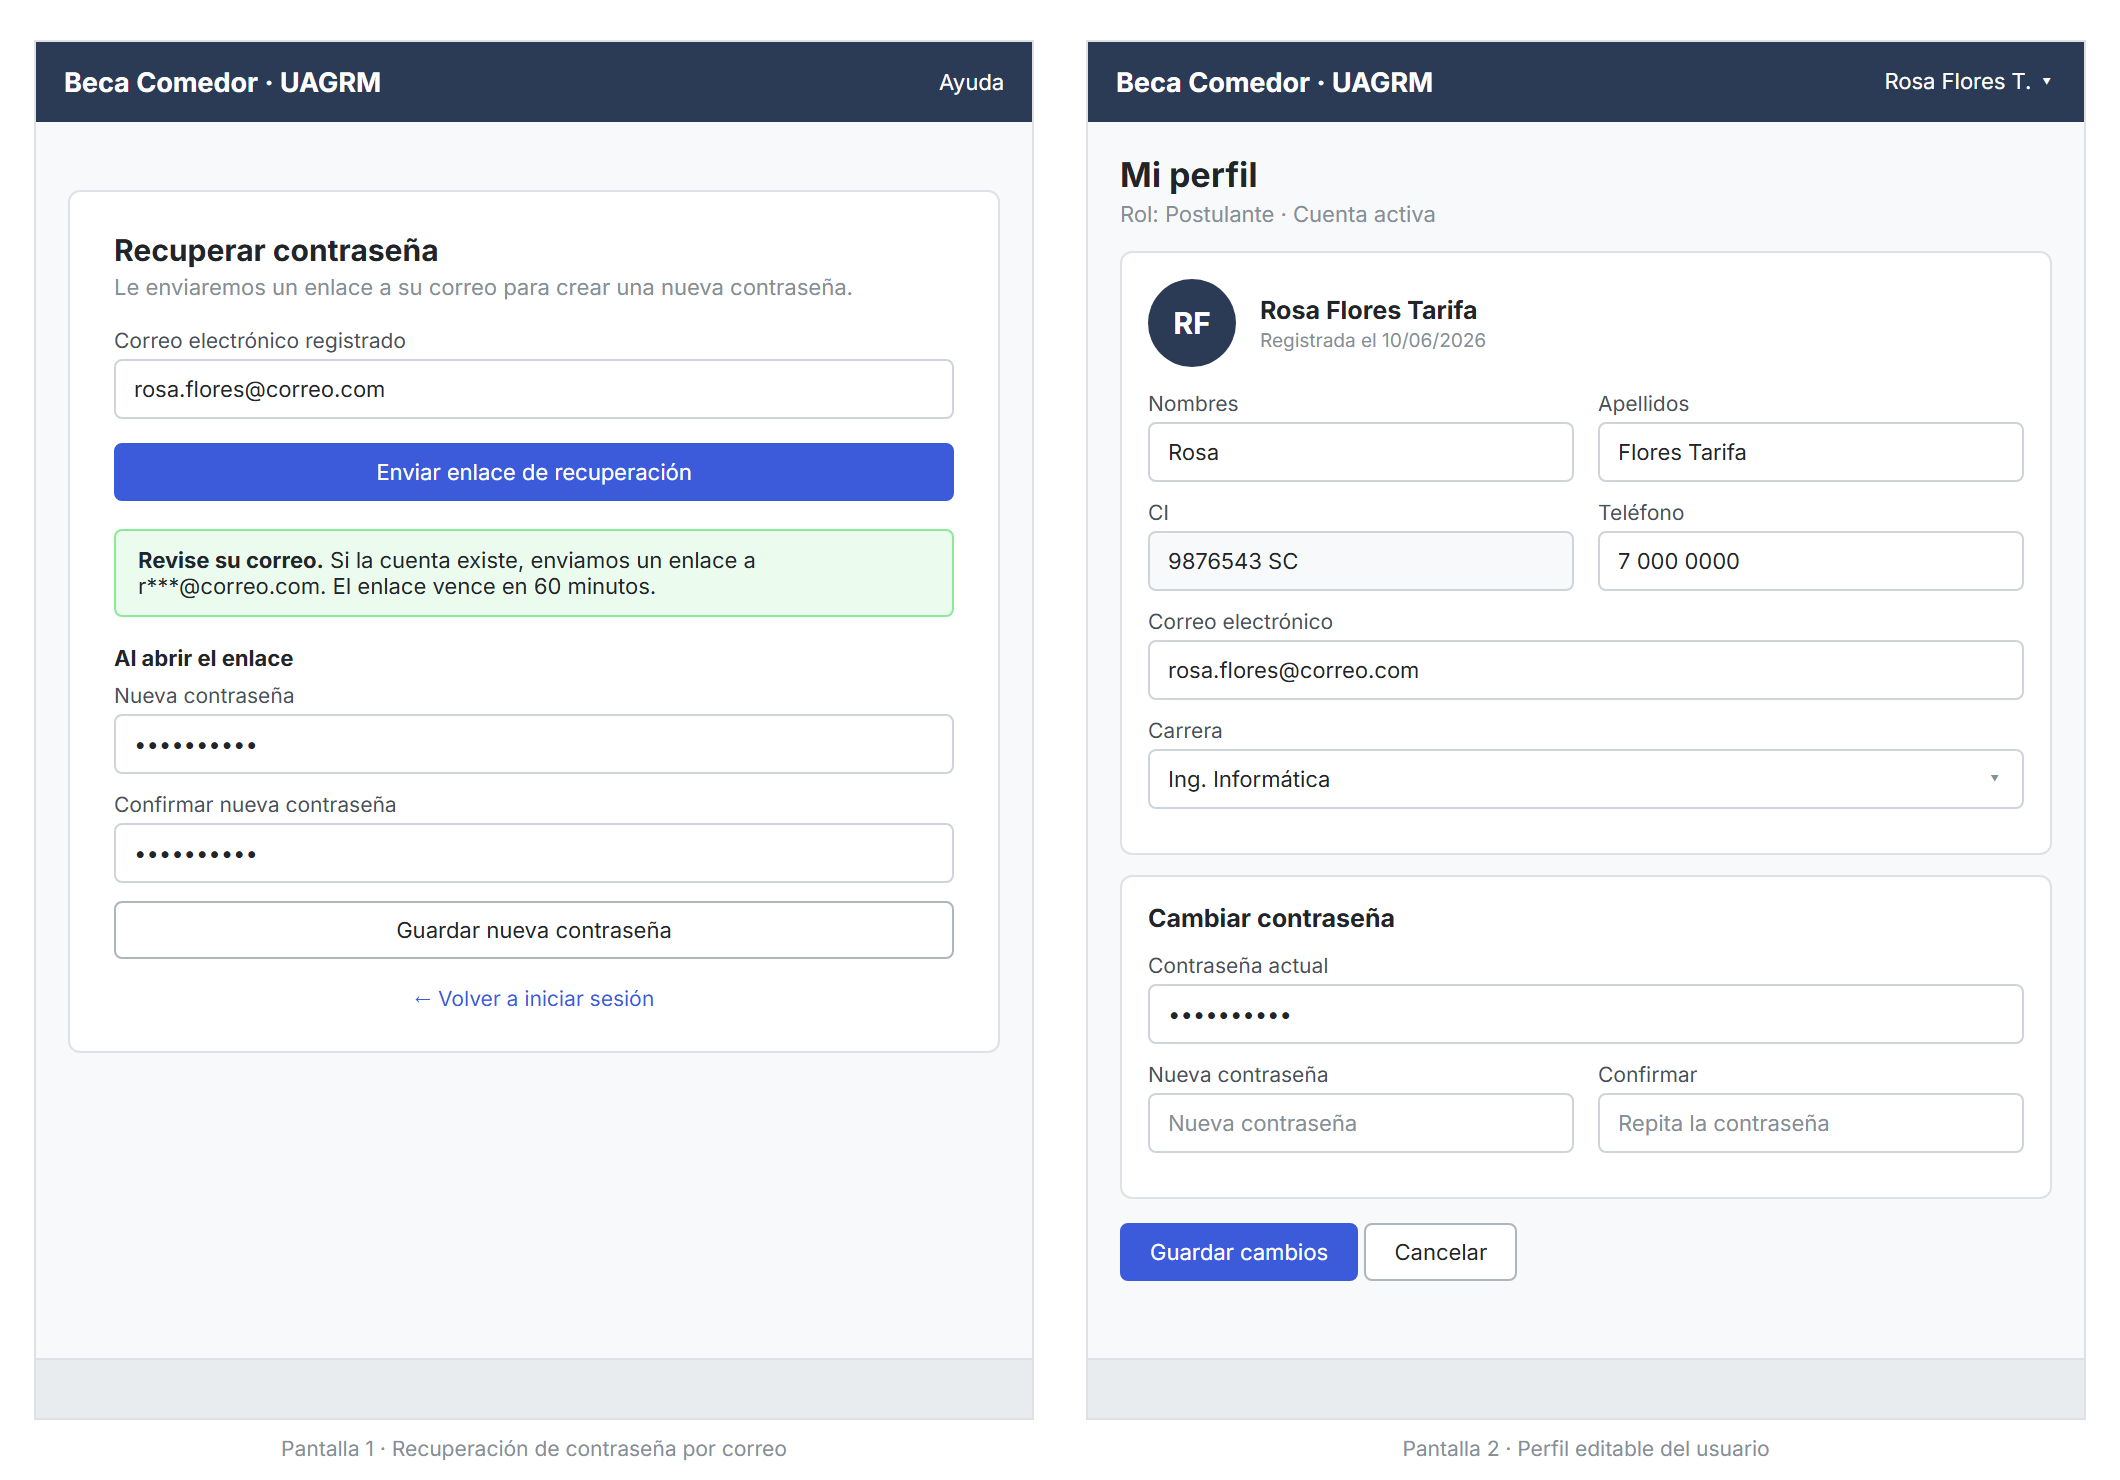
\includegraphics[width=\textwidth,height=0.75\textheight,keepaspectratio]{images/140_Mockup_CU15_Recuperar_contrasena_perfil.png}

\smallskip
\noindent\raggedright\textit{Nota.} Elaboración propia.
\end{figure}



\Needspace{0.9\textheight}
\wfb{\wn{7}.5.16. Interfaz CU-16 Digitalizar y adjuntar documentos}\label{sec:cap7_interfaz_cu16}

La Figura~\ref{fig:mockup_cu16} presenta la maqueta de interfaz del CU-16.

\begin{figure}[H]
\caption{Maqueta de interfaz del CU-16 Digitalizar y adjuntar documentos}
\label{fig:mockup_cu16}
\centering
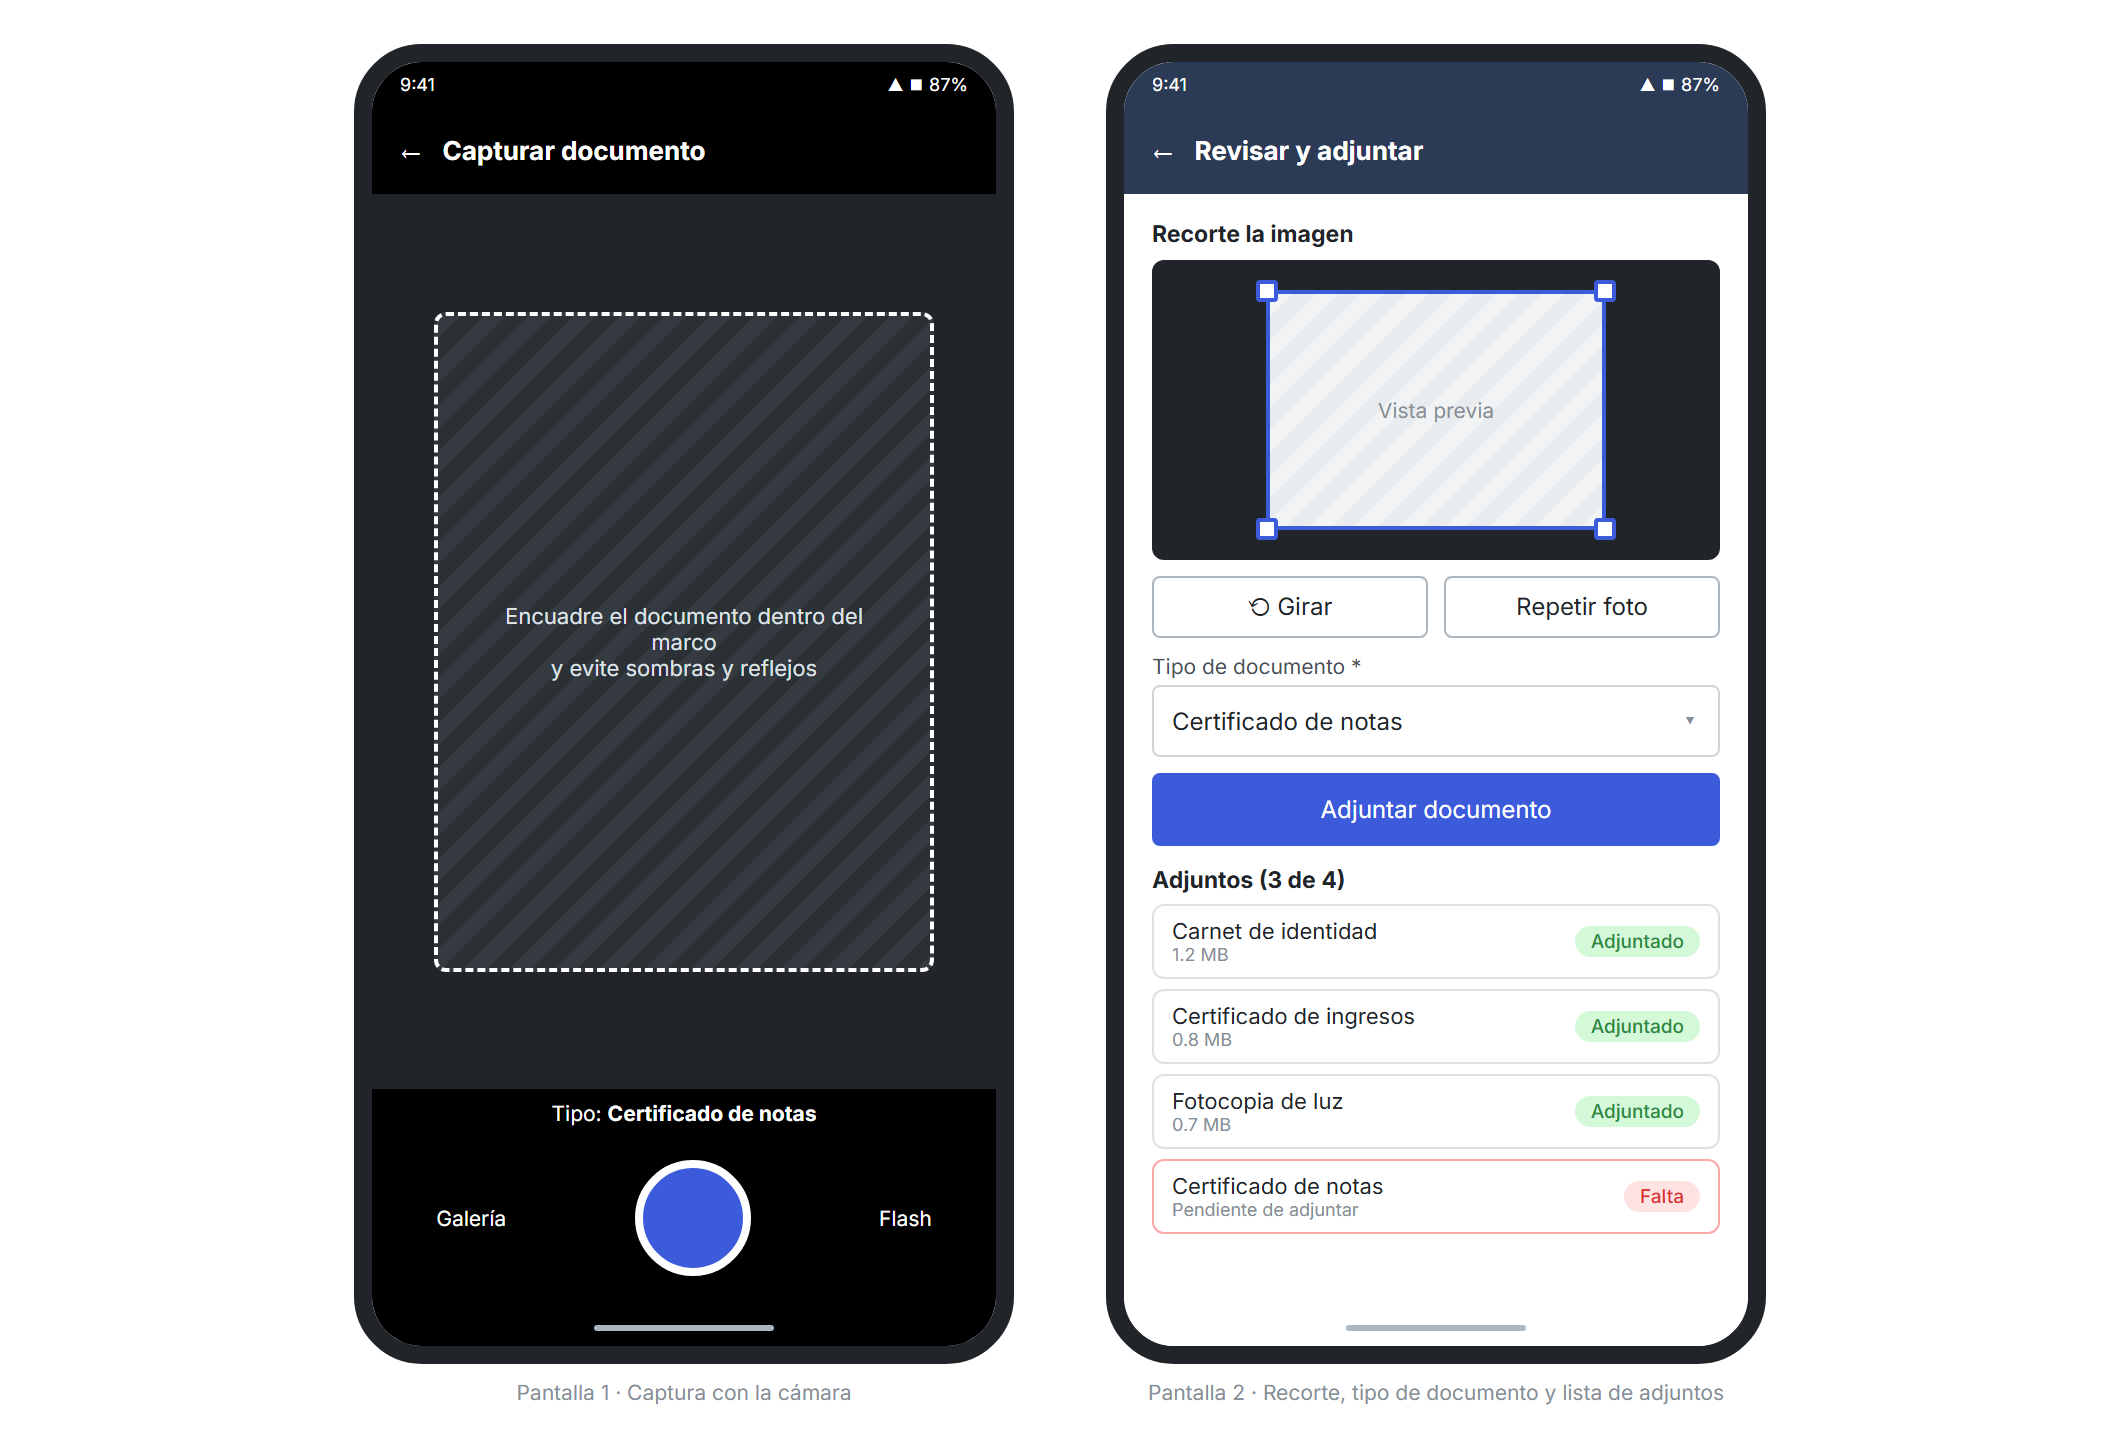
\includegraphics[width=\textwidth,height=0.75\textheight,keepaspectratio]{images/141_Mockup_CU16_Digitalizar_documentos.png}

\smallskip
\noindent\raggedright\textit{Nota.} Elaboración propia.
\end{figure}



\Needspace{0.9\textheight}
\wfb{\wn{7}.5.17. Interfaz CU-17 Guardar borrador de postulación}\label{sec:cap7_interfaz_cu17}

La Figura~\ref{fig:mockup_cu17} presenta la maqueta de interfaz del CU-17.

\begin{figure}[H]
\caption{Maqueta de interfaz del CU-17 Guardar borrador de postulación}
\label{fig:mockup_cu17}
\centering
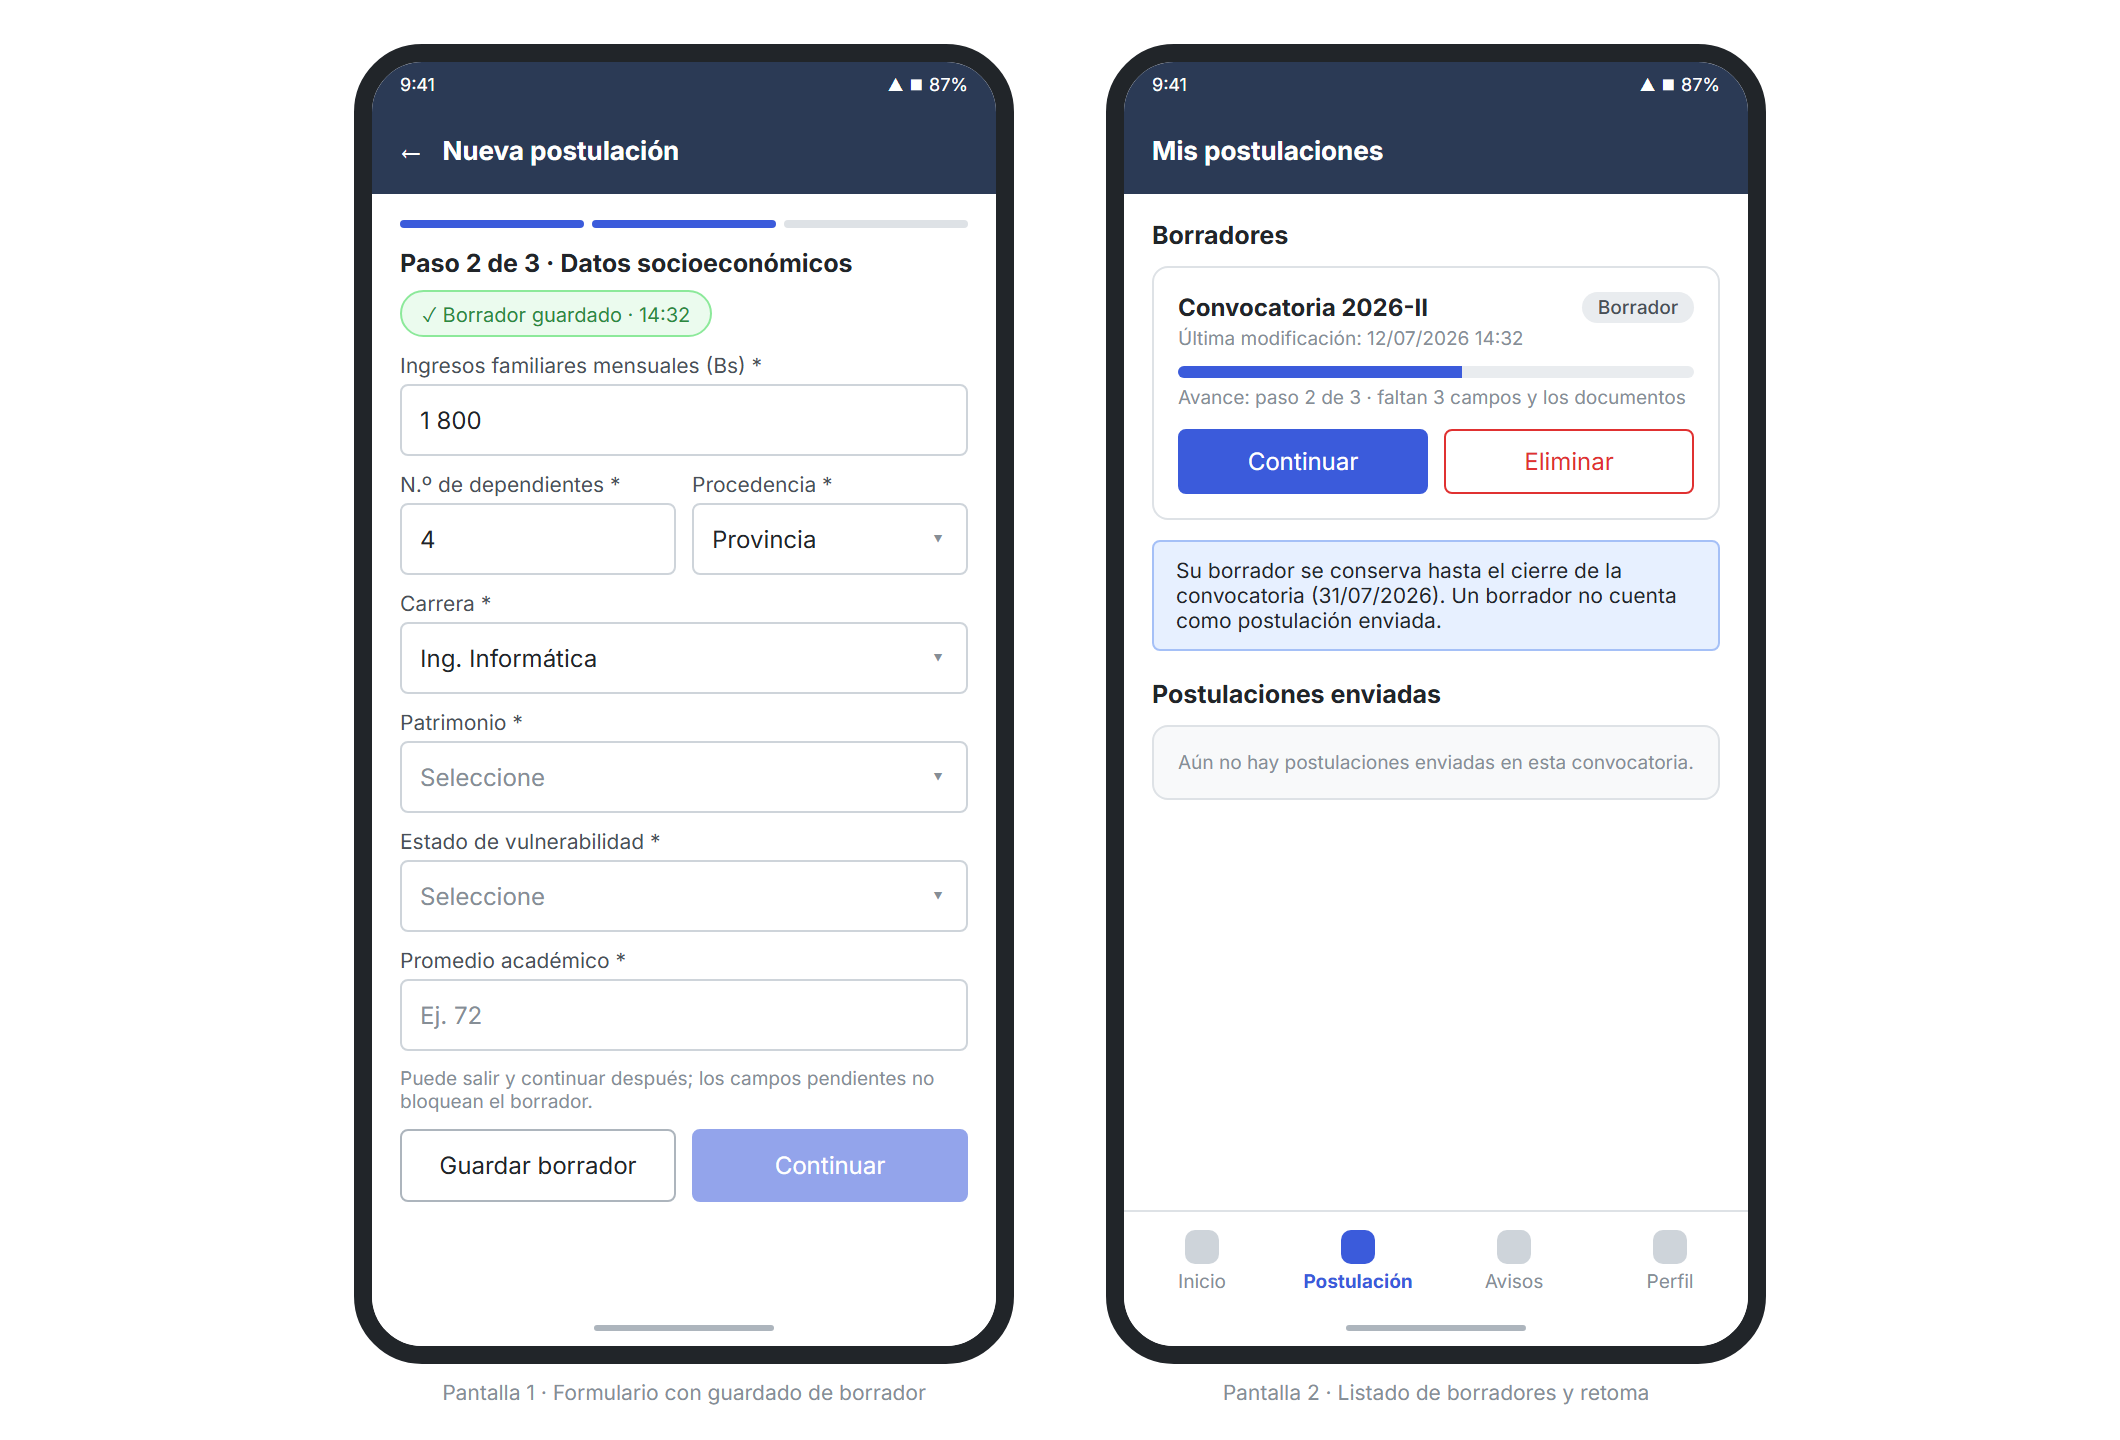
\includegraphics[width=\textwidth,height=0.75\textheight,keepaspectratio]{images/142_Mockup_CU17_Guardar_borrador.png}

\smallskip
\noindent\raggedright\textit{Nota.} Elaboración propia.
\end{figure}



\Needspace{0.9\textheight}
\wfb{\wn{7}.5.18. Interfaz CU-18 Validar elegibilidad y duplicados}\label{sec:cap7_interfaz_cu18}

La Figura~\ref{fig:mockup_cu18} presenta la maqueta de interfaz del CU-18.

\begin{figure}[H]
\caption{Maqueta de interfaz del CU-18 Validar elegibilidad y duplicados}
\label{fig:mockup_cu18}
\centering
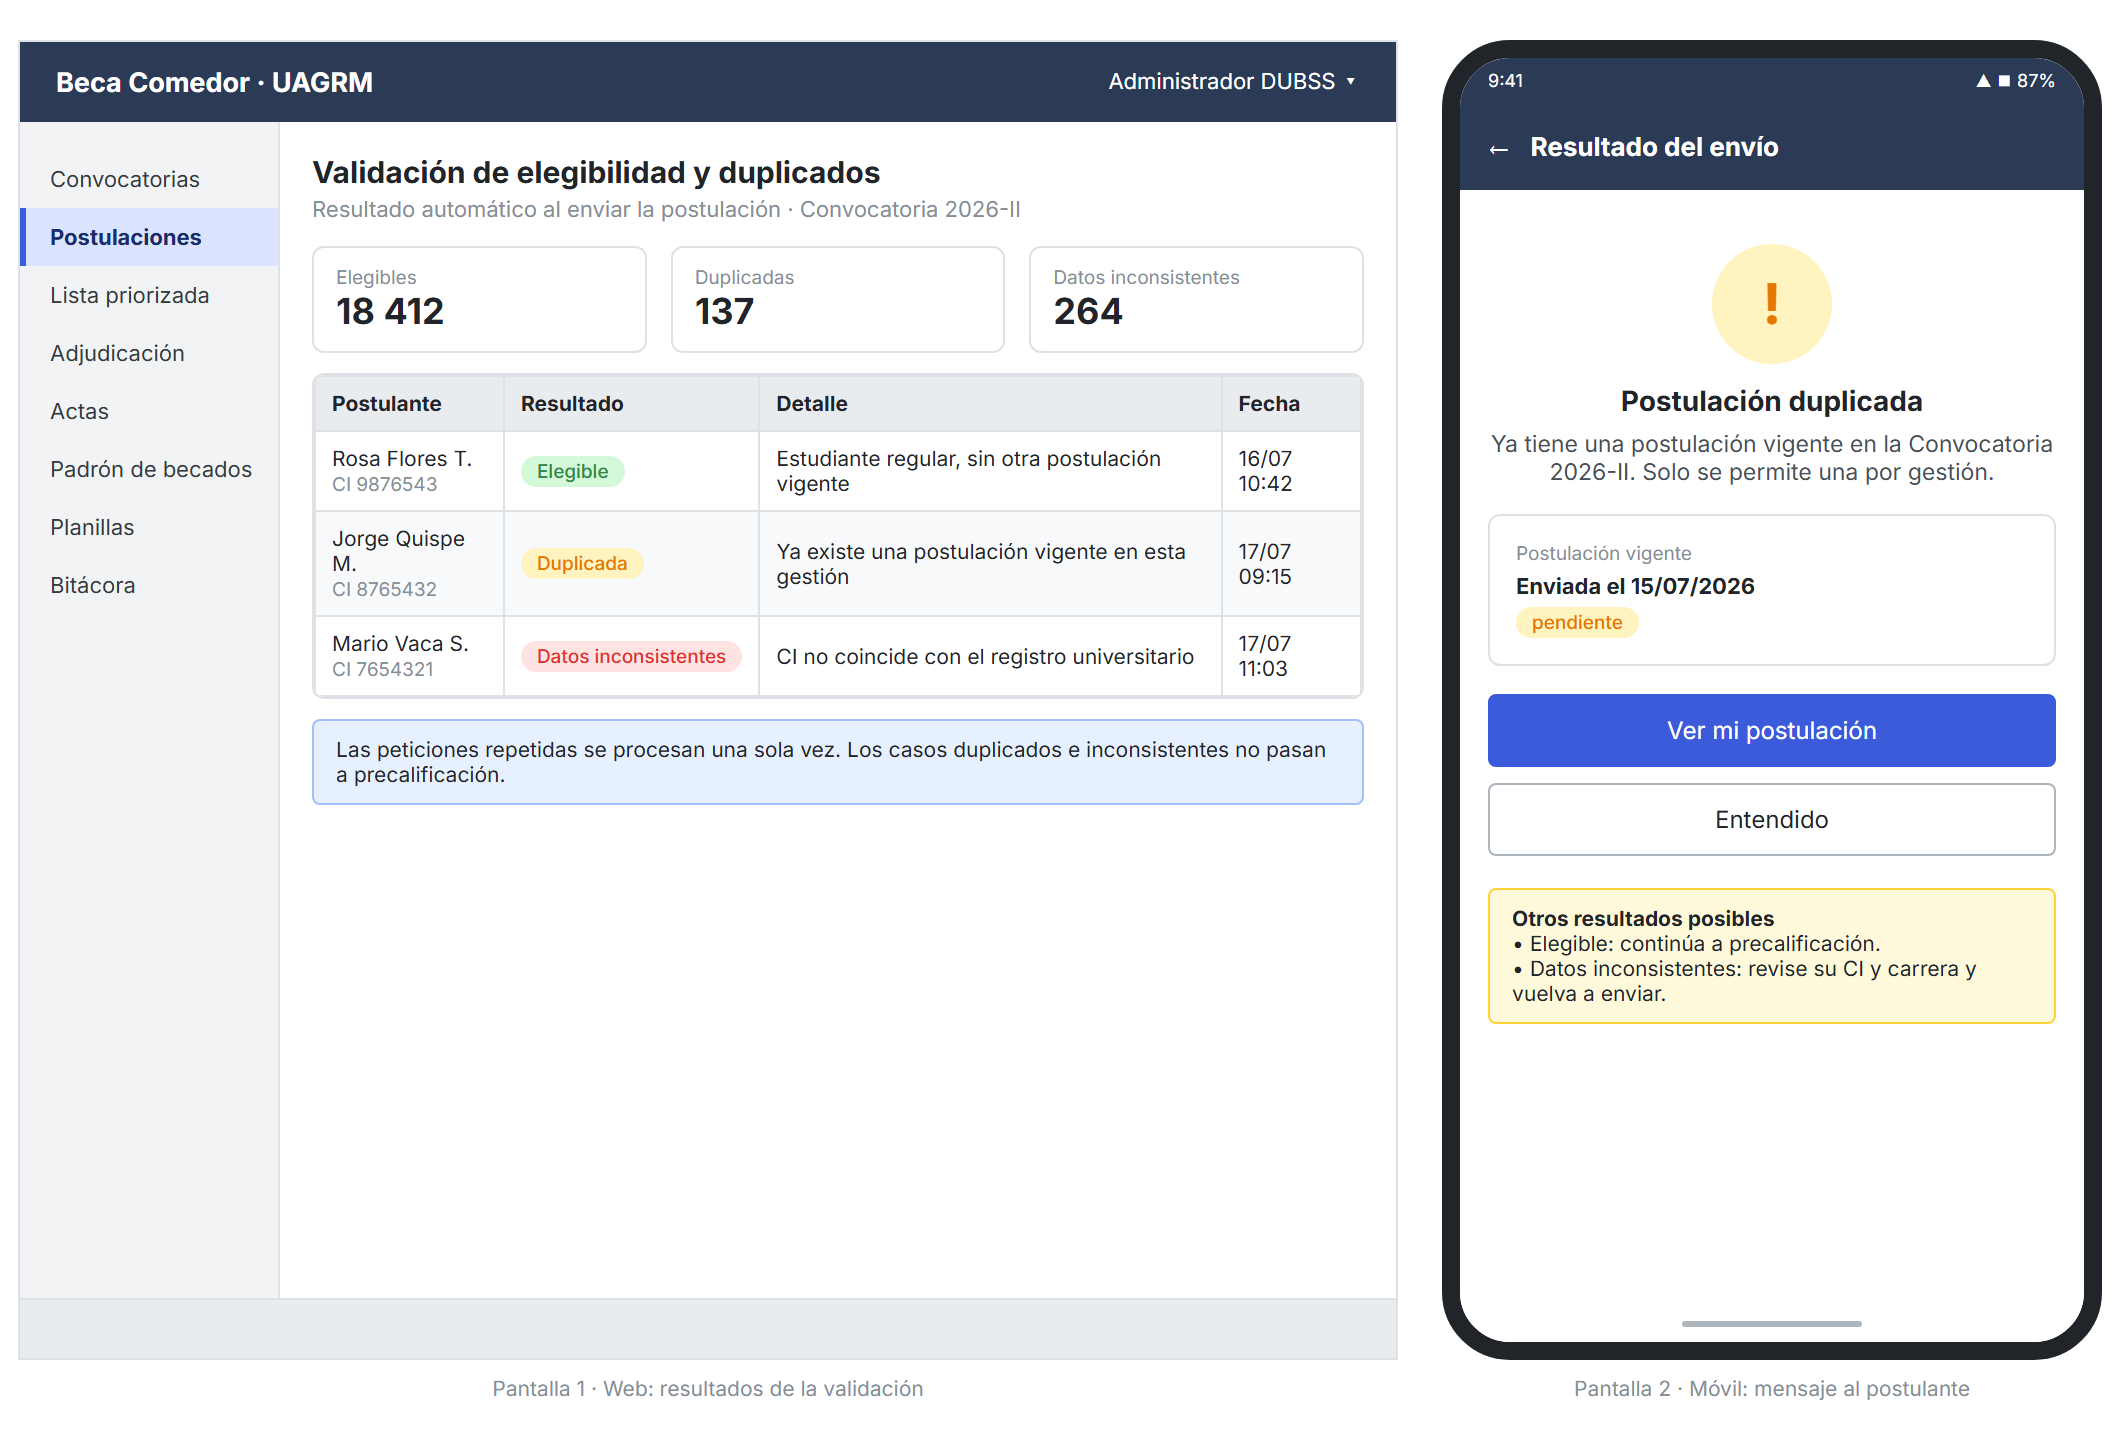
\includegraphics[width=\textwidth,height=0.75\textheight,keepaspectratio]{images/143_Mockup_CU18_Validar_elegibilidad.png}

\smallskip
\noindent\raggedright\textit{Nota.} Elaboración propia.
\end{figure}



\Needspace{0.9\textheight}
\wfb{\wn{7}.5.19. Interfaz CU-19 Devolver postulación para corrección}\label{sec:cap7_interfaz_cu19}

La Figura~\ref{fig:mockup_cu19} presenta la maqueta de interfaz del CU-19.

\begin{figure}[H]
\caption{Maqueta de interfaz del CU-19 Devolver postulación para corrección}
\label{fig:mockup_cu19}
\centering
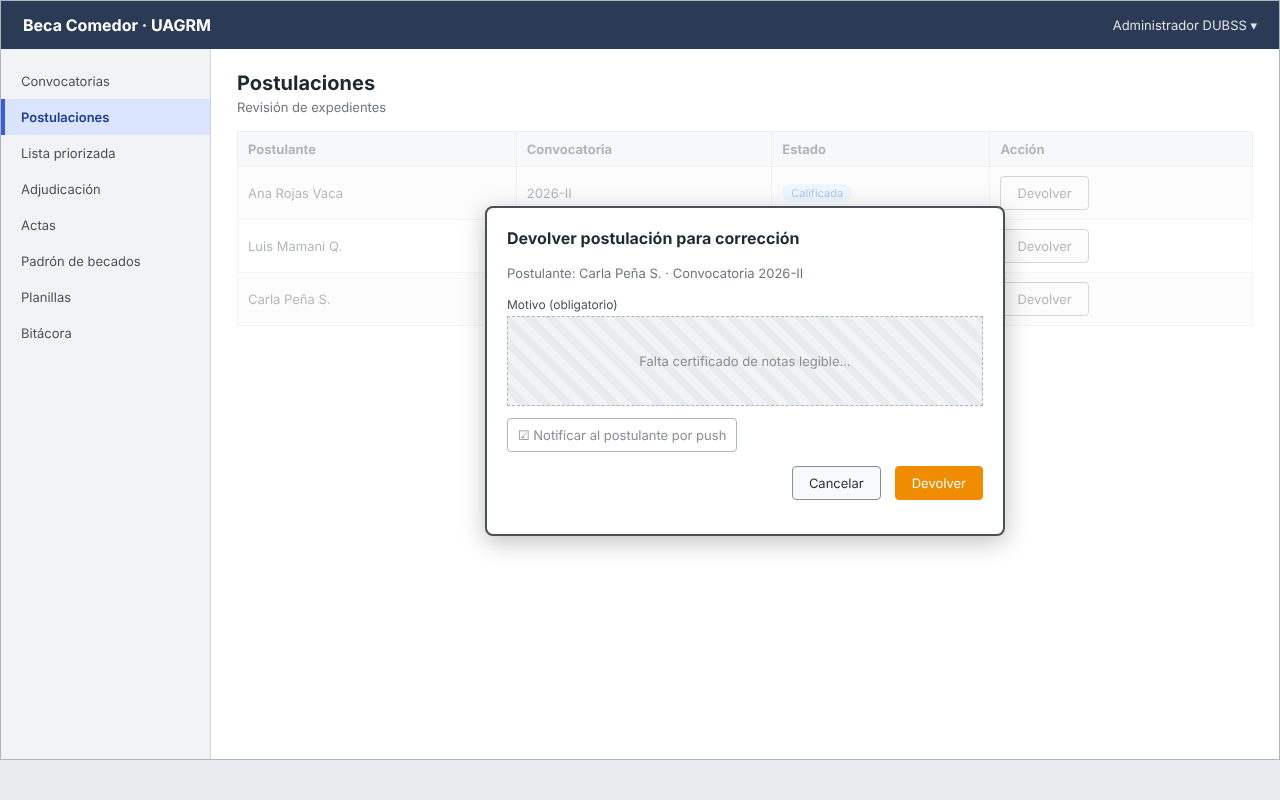
\includegraphics[width=\textwidth,height=0.75\textheight,keepaspectratio]{images/113_Mockup_CU19_Devolver_para_correccion.png}

\smallskip
\noindent\raggedright\textit{Nota.} Elaboración propia.
\end{figure}


\Needspace{0.9\textheight}
\wfb{\wn{7}.5.20. Interfaz CU-20 Archivar o rechazar postulación}\label{sec:cap7_interfaz_cu20}

La Figura~\ref{fig:mockup_cu20} presenta la maqueta de interfaz del CU-20.

\begin{figure}[H]
\caption{Maqueta de interfaz del CU-20 Archivar o rechazar postulación}
\label{fig:mockup_cu20}
\centering
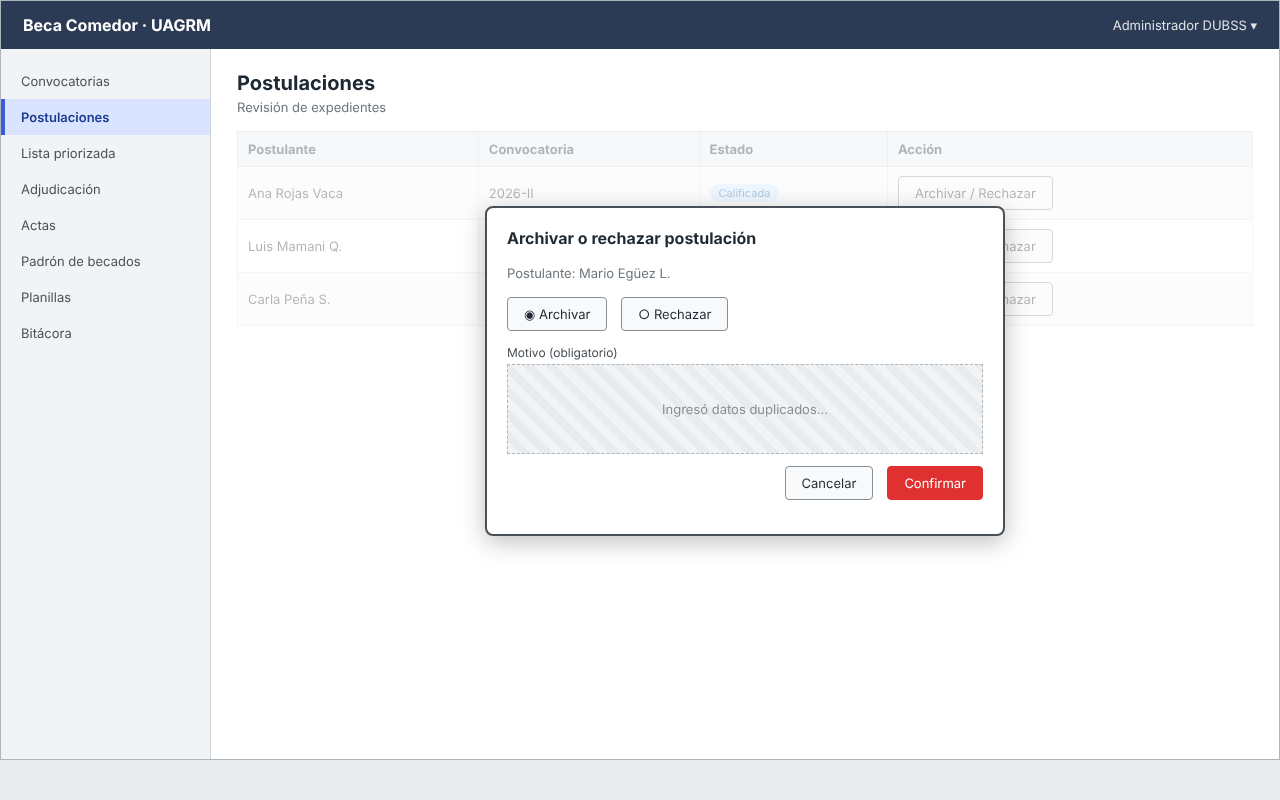
\includegraphics[width=\textwidth,height=0.75\textheight,keepaspectratio]{images/114_Mockup_CU20_Archivar_o_rechazar_postulacion.png}

\smallskip
\noindent\raggedright\textit{Nota.} Elaboración propia.
\end{figure}


\Needspace{0.9\textheight}
\wfb{\wn{7}.5.21. Interfaz CU-21 Notificar finalistas, registrar entrega de documentación física y publicar comunicados/avisos}\label{sec:cap7_interfaz_cu21}

La Figura~\ref{fig:mockup_cu21} presenta la maqueta de interfaz del CU-21.

\begin{figure}[H]
\caption{Maqueta de interfaz del CU-21 Notificar finalistas, registrar entrega de documentación física y publicar comunicados/avisos}
\label{fig:mockup_cu21}
\centering
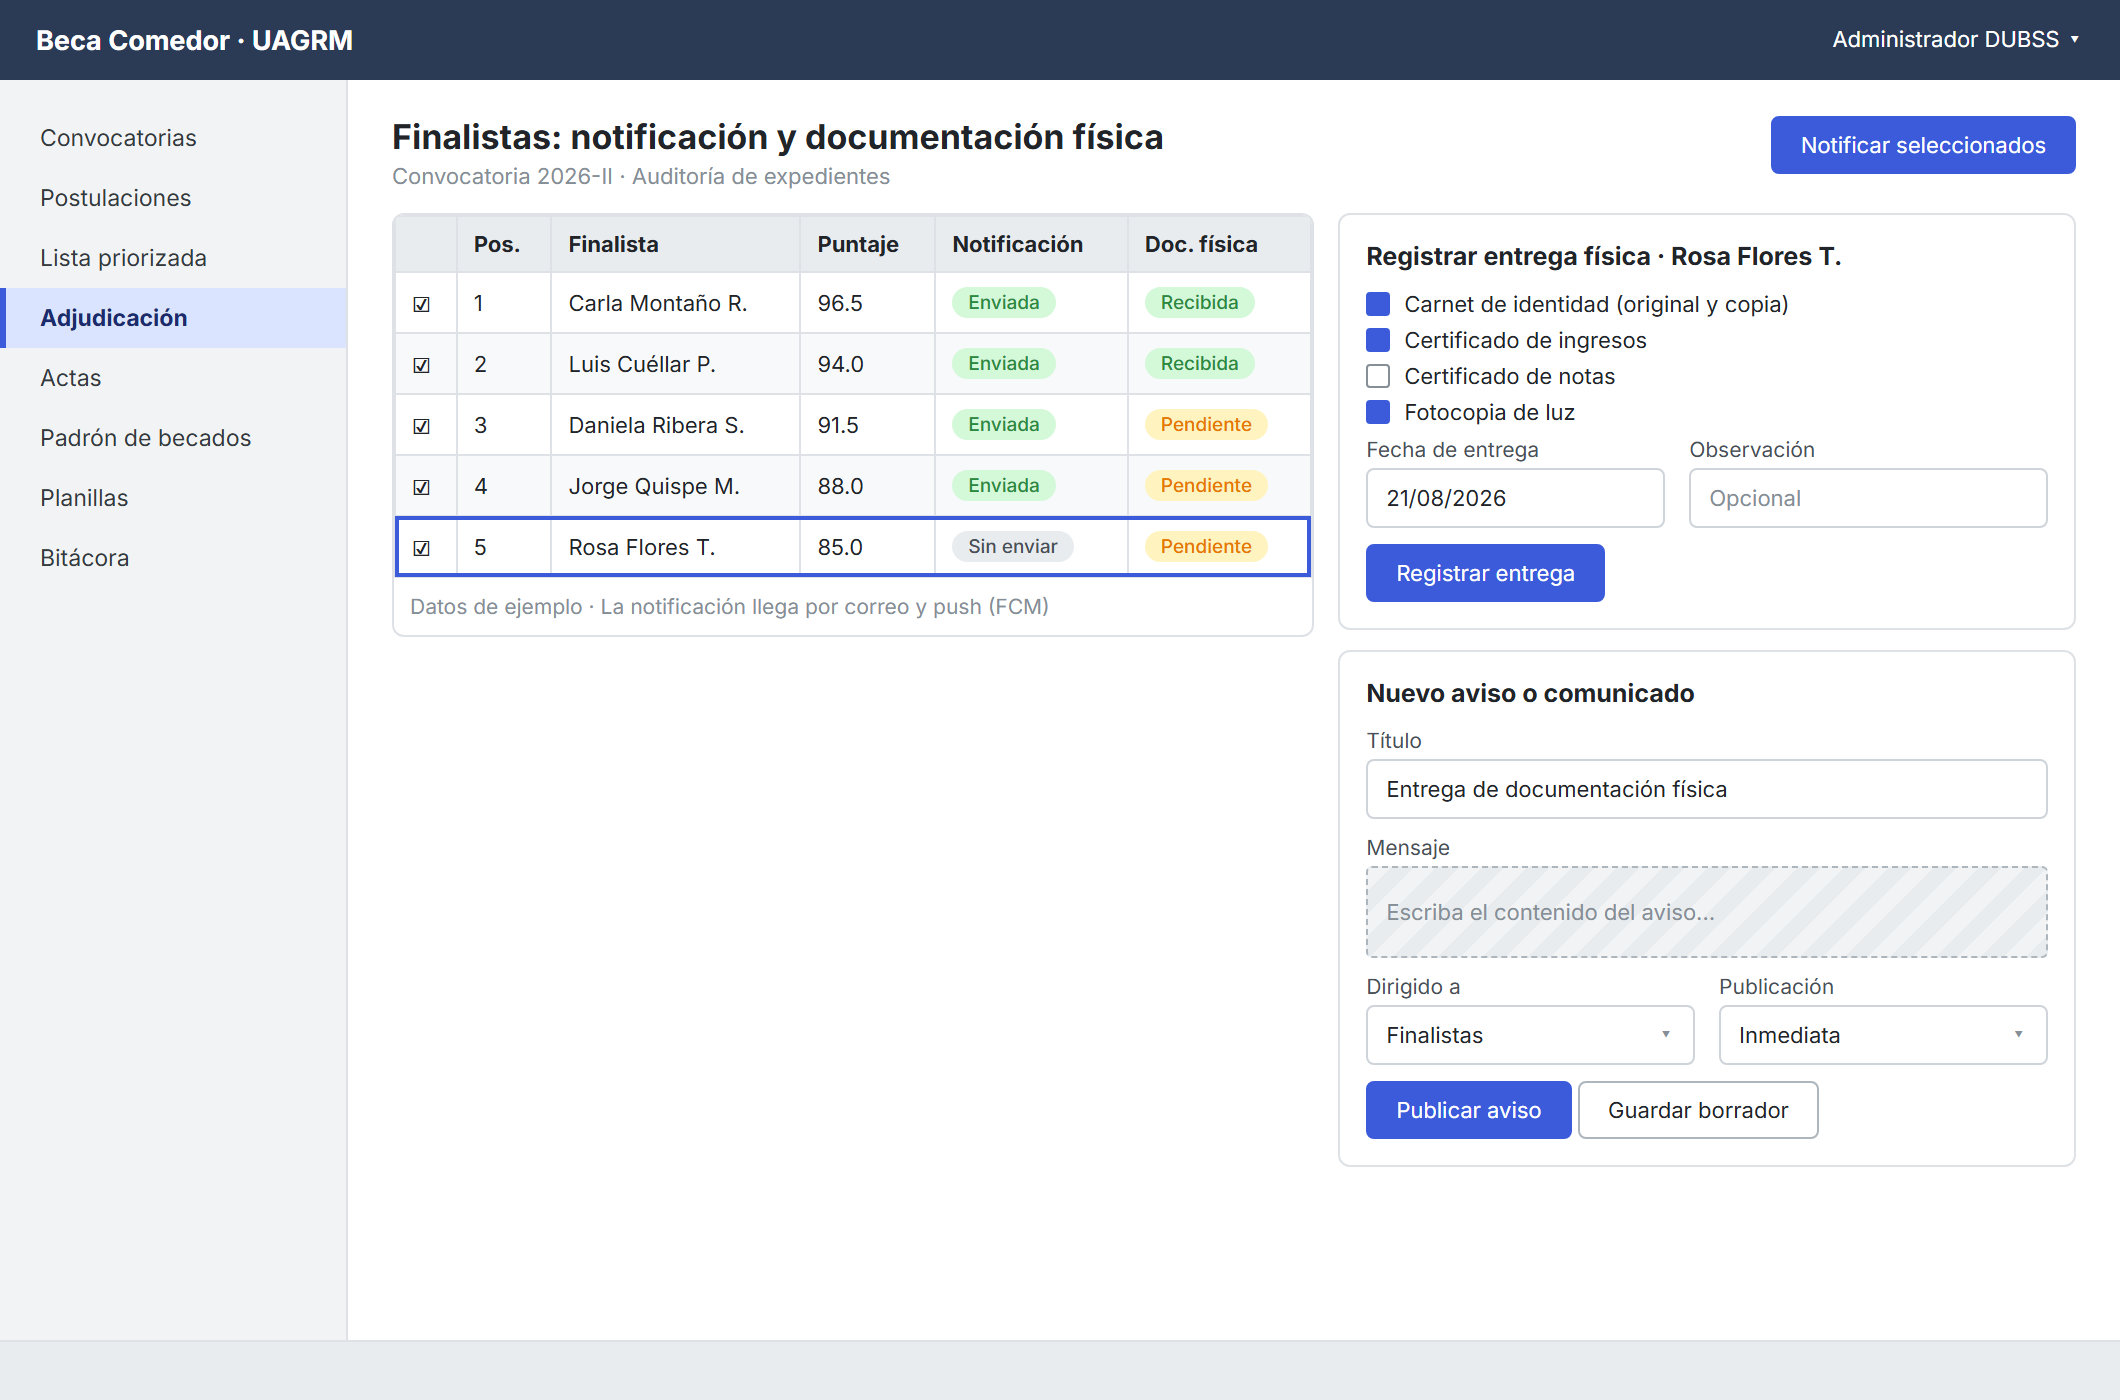
\includegraphics[width=\textwidth,height=0.75\textheight,keepaspectratio]{images/144_Mockup_CU21_Notificar_finalistas_avisos.png}

\smallskip
\noindent\raggedright\textit{Nota.} Elaboración propia.
\end{figure}



\Needspace{0.9\textheight}
\wfb{\wn{7}.5.22. Interfaz CU-22 Publicar resultados de adjudicación}\label{sec:cap7_interfaz_cu22}

La Figura~\ref{fig:mockup_cu22} presenta la maqueta de interfaz del CU-22.

\begin{figure}[H]
\caption{Maqueta de interfaz del CU-22 Publicar resultados de adjudicación}
\label{fig:mockup_cu22}
\centering
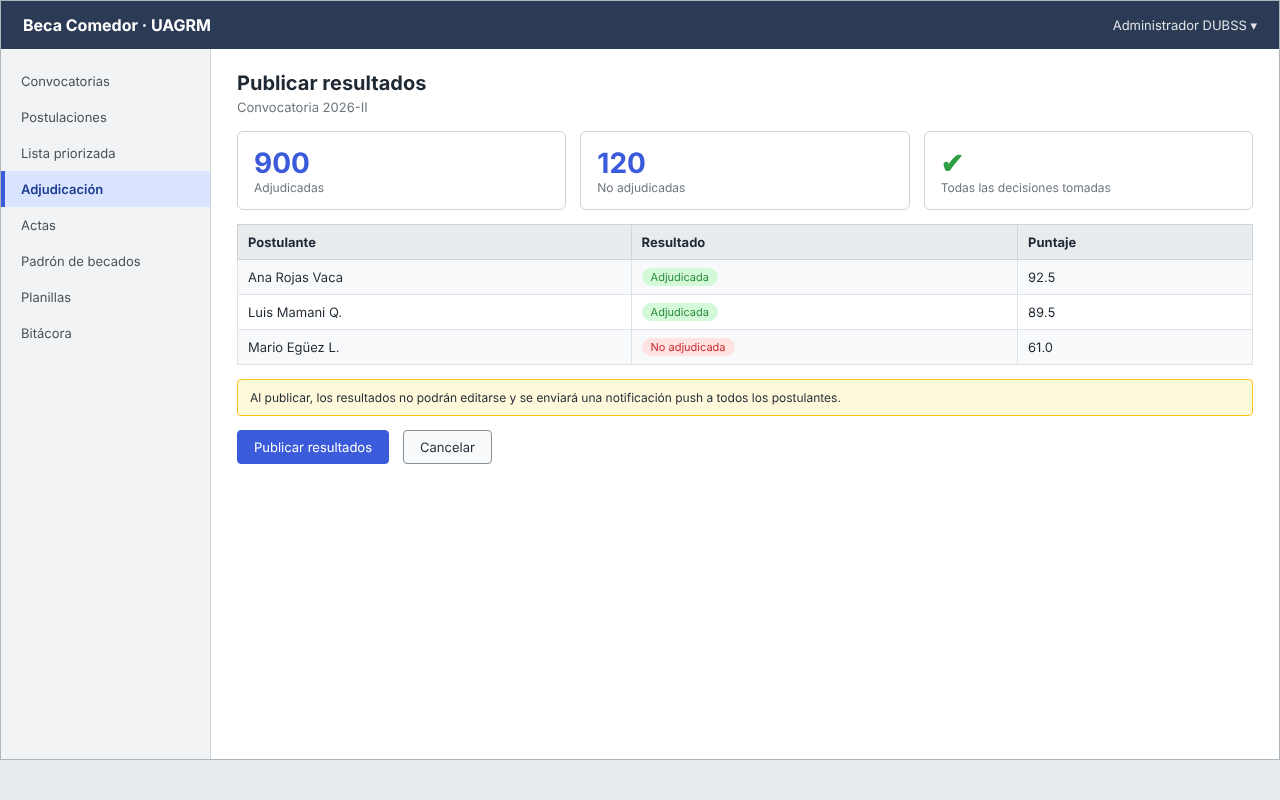
\includegraphics[width=\textwidth,height=0.75\textheight,keepaspectratio]{images/115_Mockup_CU22_Publicar_resultados.png}

\smallskip
\noindent\raggedright\textit{Nota.} Elaboración propia.
\end{figure}


\Needspace{0.9\textheight}
\wfb{\wn{7}.5.23. Interfaz CU-23 Gestionar padrón de becados (baja, suspensión, reemplazo)}\label{sec:cap7_interfaz_cu23}

La Figura~\ref{fig:mockup_cu23} presenta la maqueta de interfaz del CU-23.

\begin{figure}[H]
\caption{Maqueta de interfaz del CU-23 Gestionar padrón de becados (baja, suspensión, reemplazo)}
\label{fig:mockup_cu23}
\centering
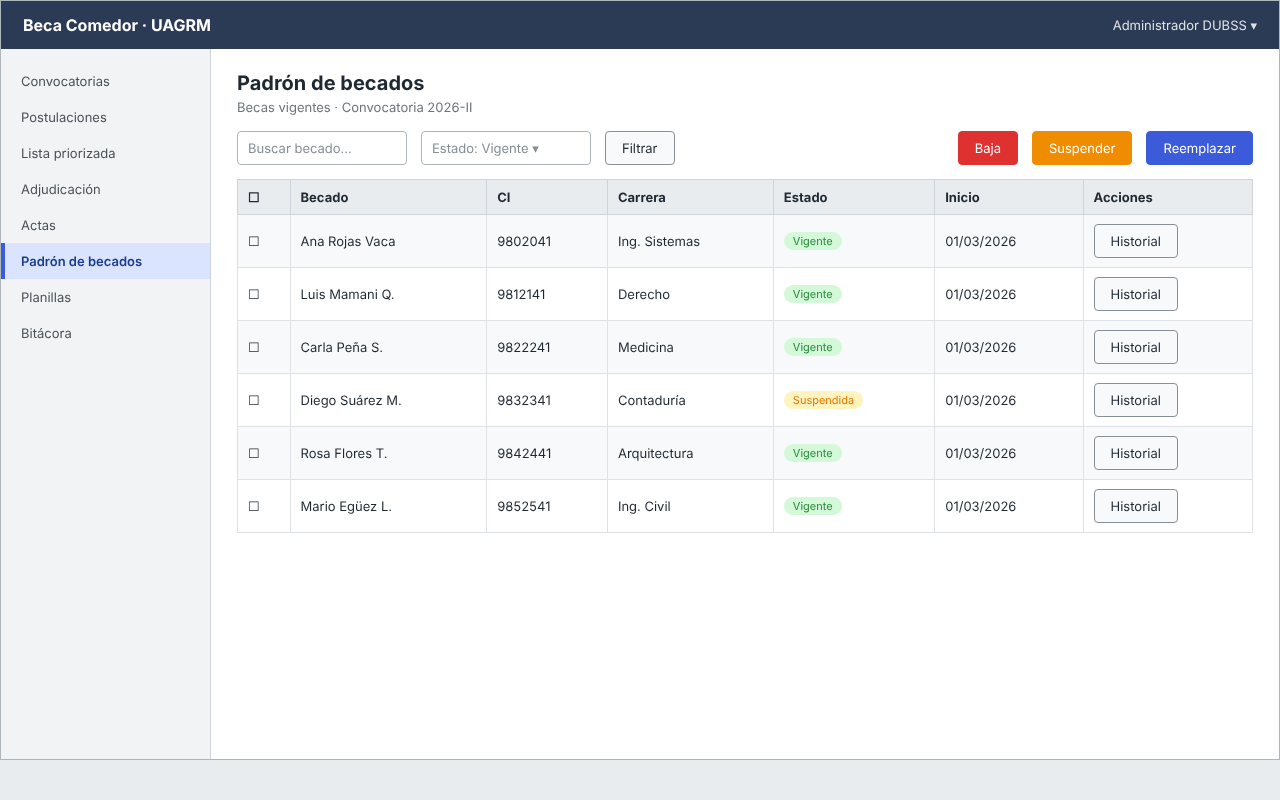
\includegraphics[width=\textwidth,height=0.75\textheight,keepaspectratio]{images/116_Mockup_CU23_Padron_de_becados.png}

\smallskip
\noindent\raggedright\textit{Nota.} Elaboración propia.
\end{figure}


\Needspace{0.9\textheight}
\wfb{\wn{7}.5.24. Interfaz CU-24 Consultar historial de asistencia y estado de beca}\label{sec:cap7_interfaz_cu24}

La Figura~\ref{fig:mockup_cu24} presenta la maqueta de interfaz del CU-24.

\begin{figure}[H]
\caption{Maqueta de interfaz del CU-24 Consultar historial de asistencia y estado de beca}
\label{fig:mockup_cu24}
\centering
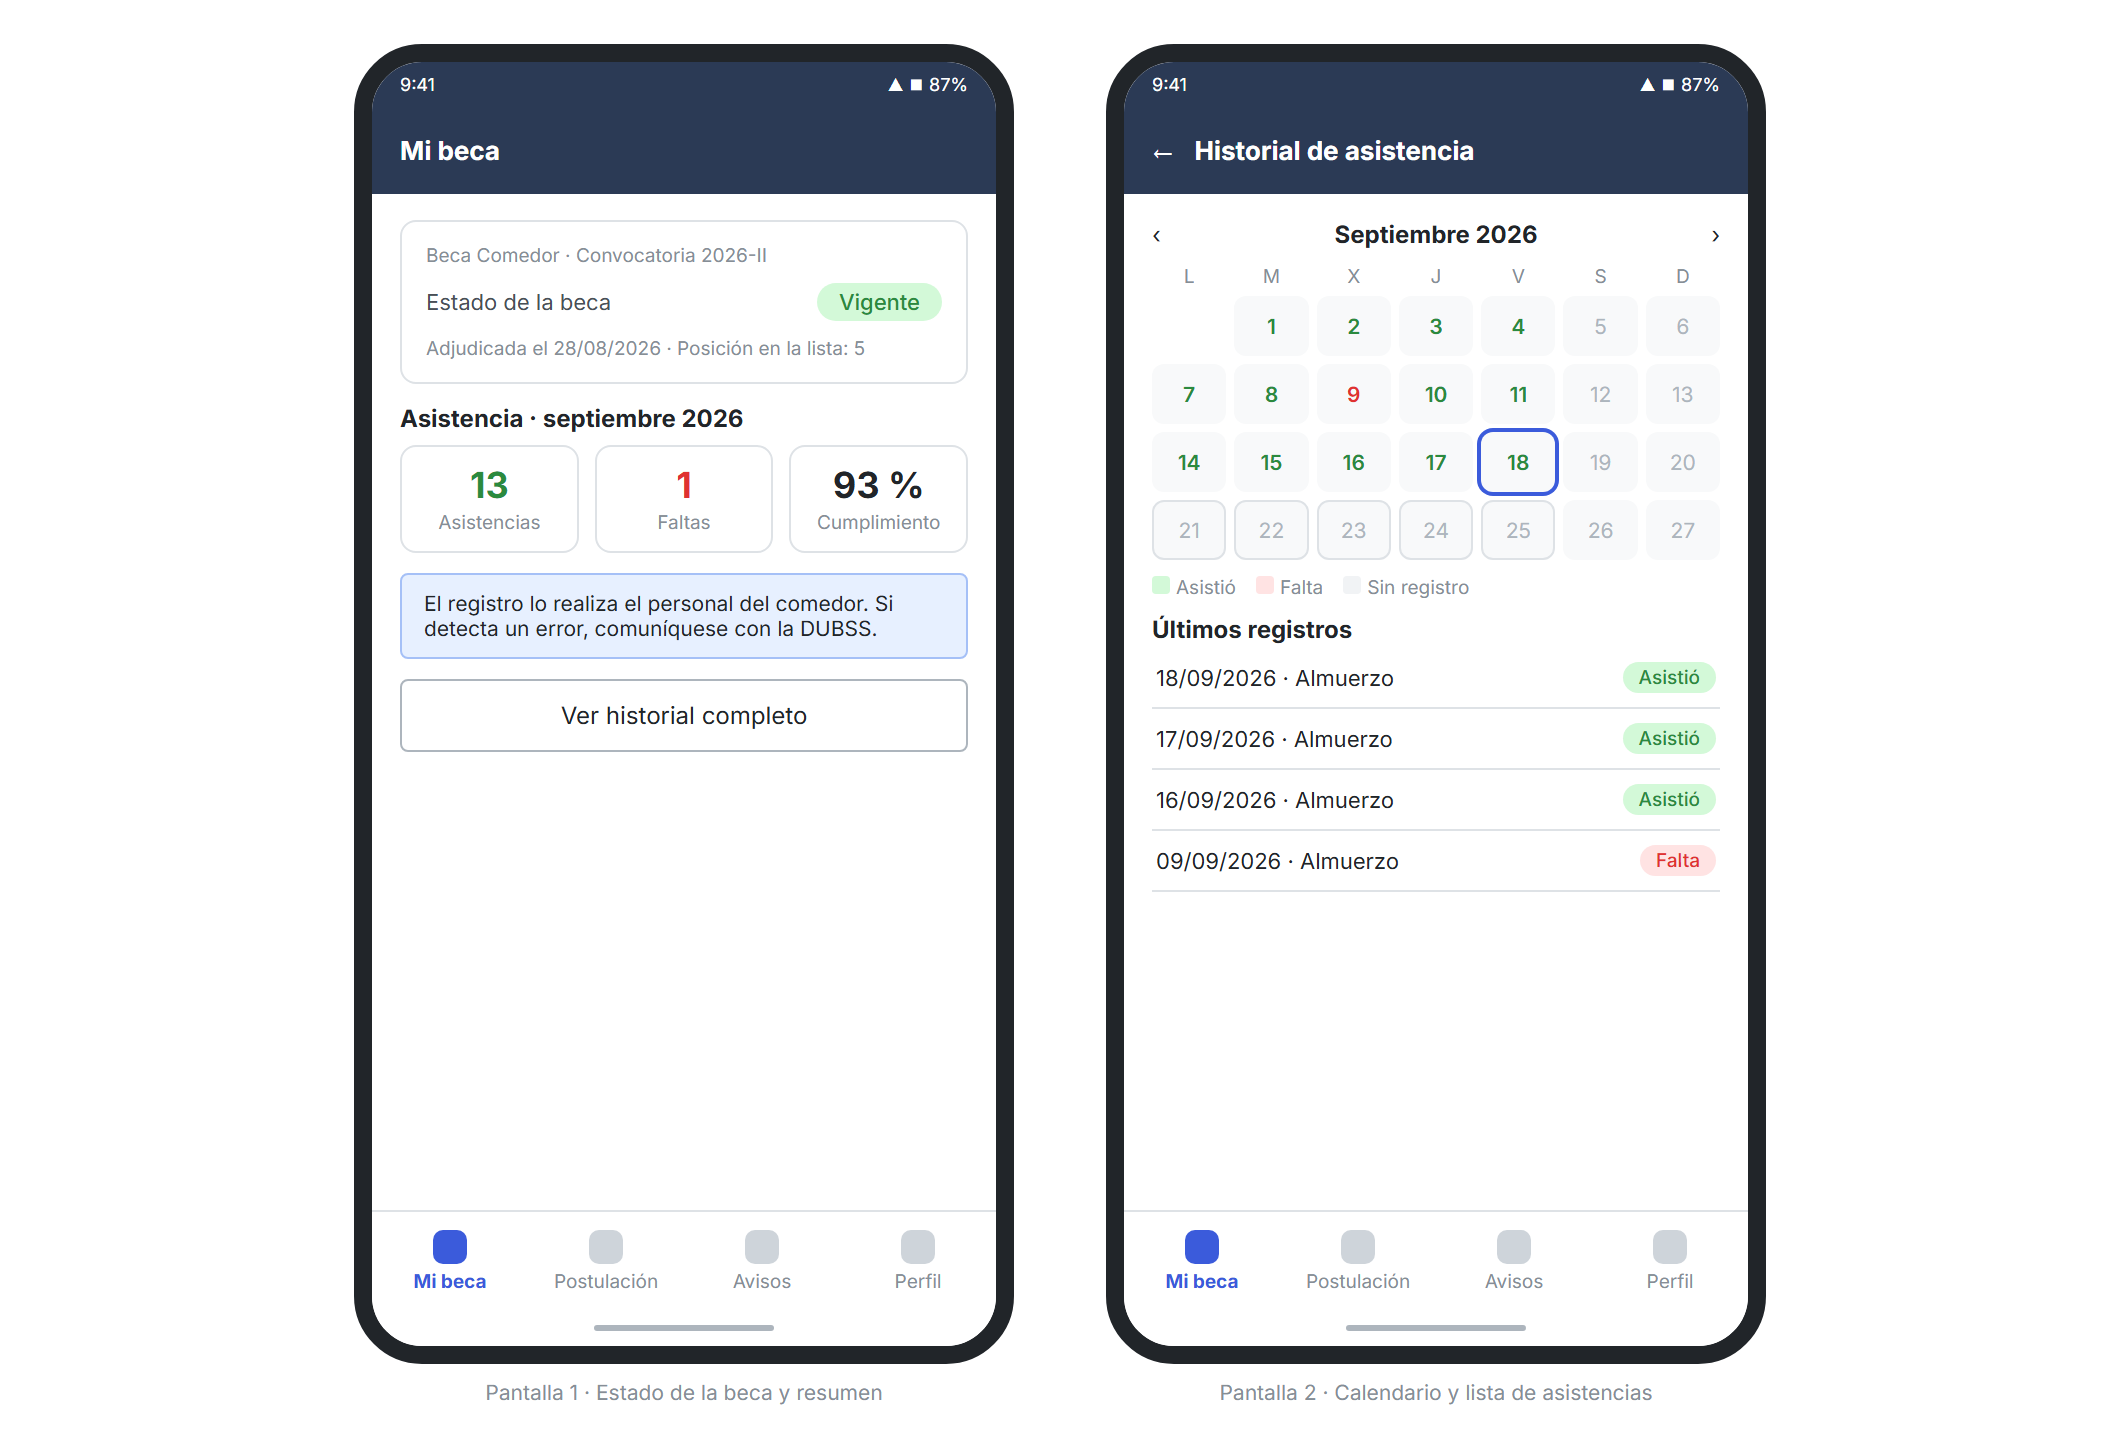
\includegraphics[width=\textwidth,height=0.75\textheight,keepaspectratio]{images/145_Mockup_CU24_Historial_asistencia.png}

\smallskip
\noindent\raggedright\textit{Nota.} Elaboración propia.
\end{figure}



\Needspace{0.9\textheight}
\wfb{\wn{7}.5.25. Interfaz CU-25 Consultar bitácora de acciones}\label{sec:cap7_interfaz_cu25}

La Figura~\ref{fig:mockup_cu25} presenta la maqueta de interfaz del CU-25.

\begin{figure}[H]
\caption{Maqueta de interfaz del CU-25 Consultar bitácora de acciones}
\label{fig:mockup_cu25}
\centering
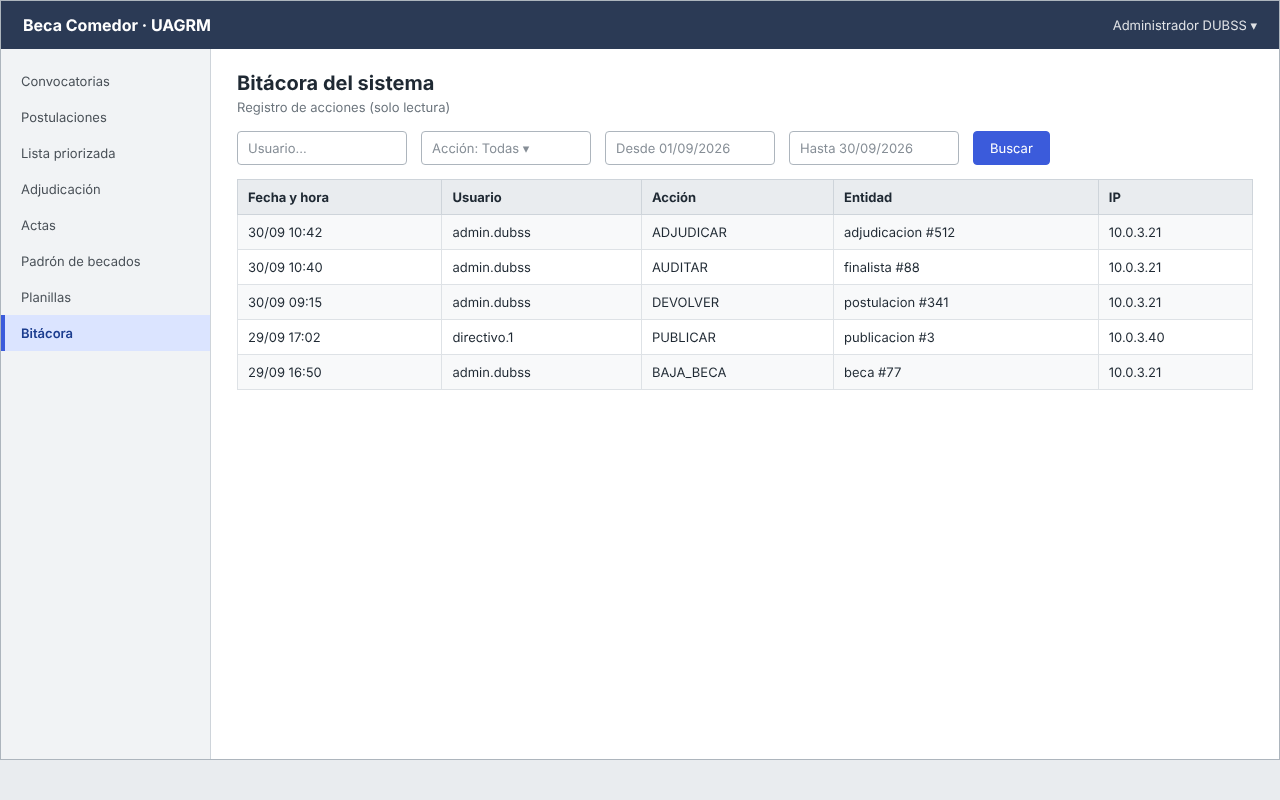
\includegraphics[width=\textwidth,height=0.75\textheight,keepaspectratio]{images/117_Mockup_CU25_Bitacora.png}

\smallskip
\noindent\raggedright\textit{Nota.} Elaboración propia.
\end{figure}


\Needspace{0.9\textheight}
\wfb{\wn{7}.5.26. Interfaz CU-26 Parametrizar modelo de preselección y reprocesar puntajes}\label{sec:cap7_interfaz_cu26}

La Figura~\ref{fig:mockup_cu26} presenta la maqueta de interfaz del CU-26.

\begin{figure}[H]
\caption{Maqueta de interfaz del CU-26 Parametrizar modelo de preselección y reprocesar puntajes}
\label{fig:mockup_cu26}
\centering
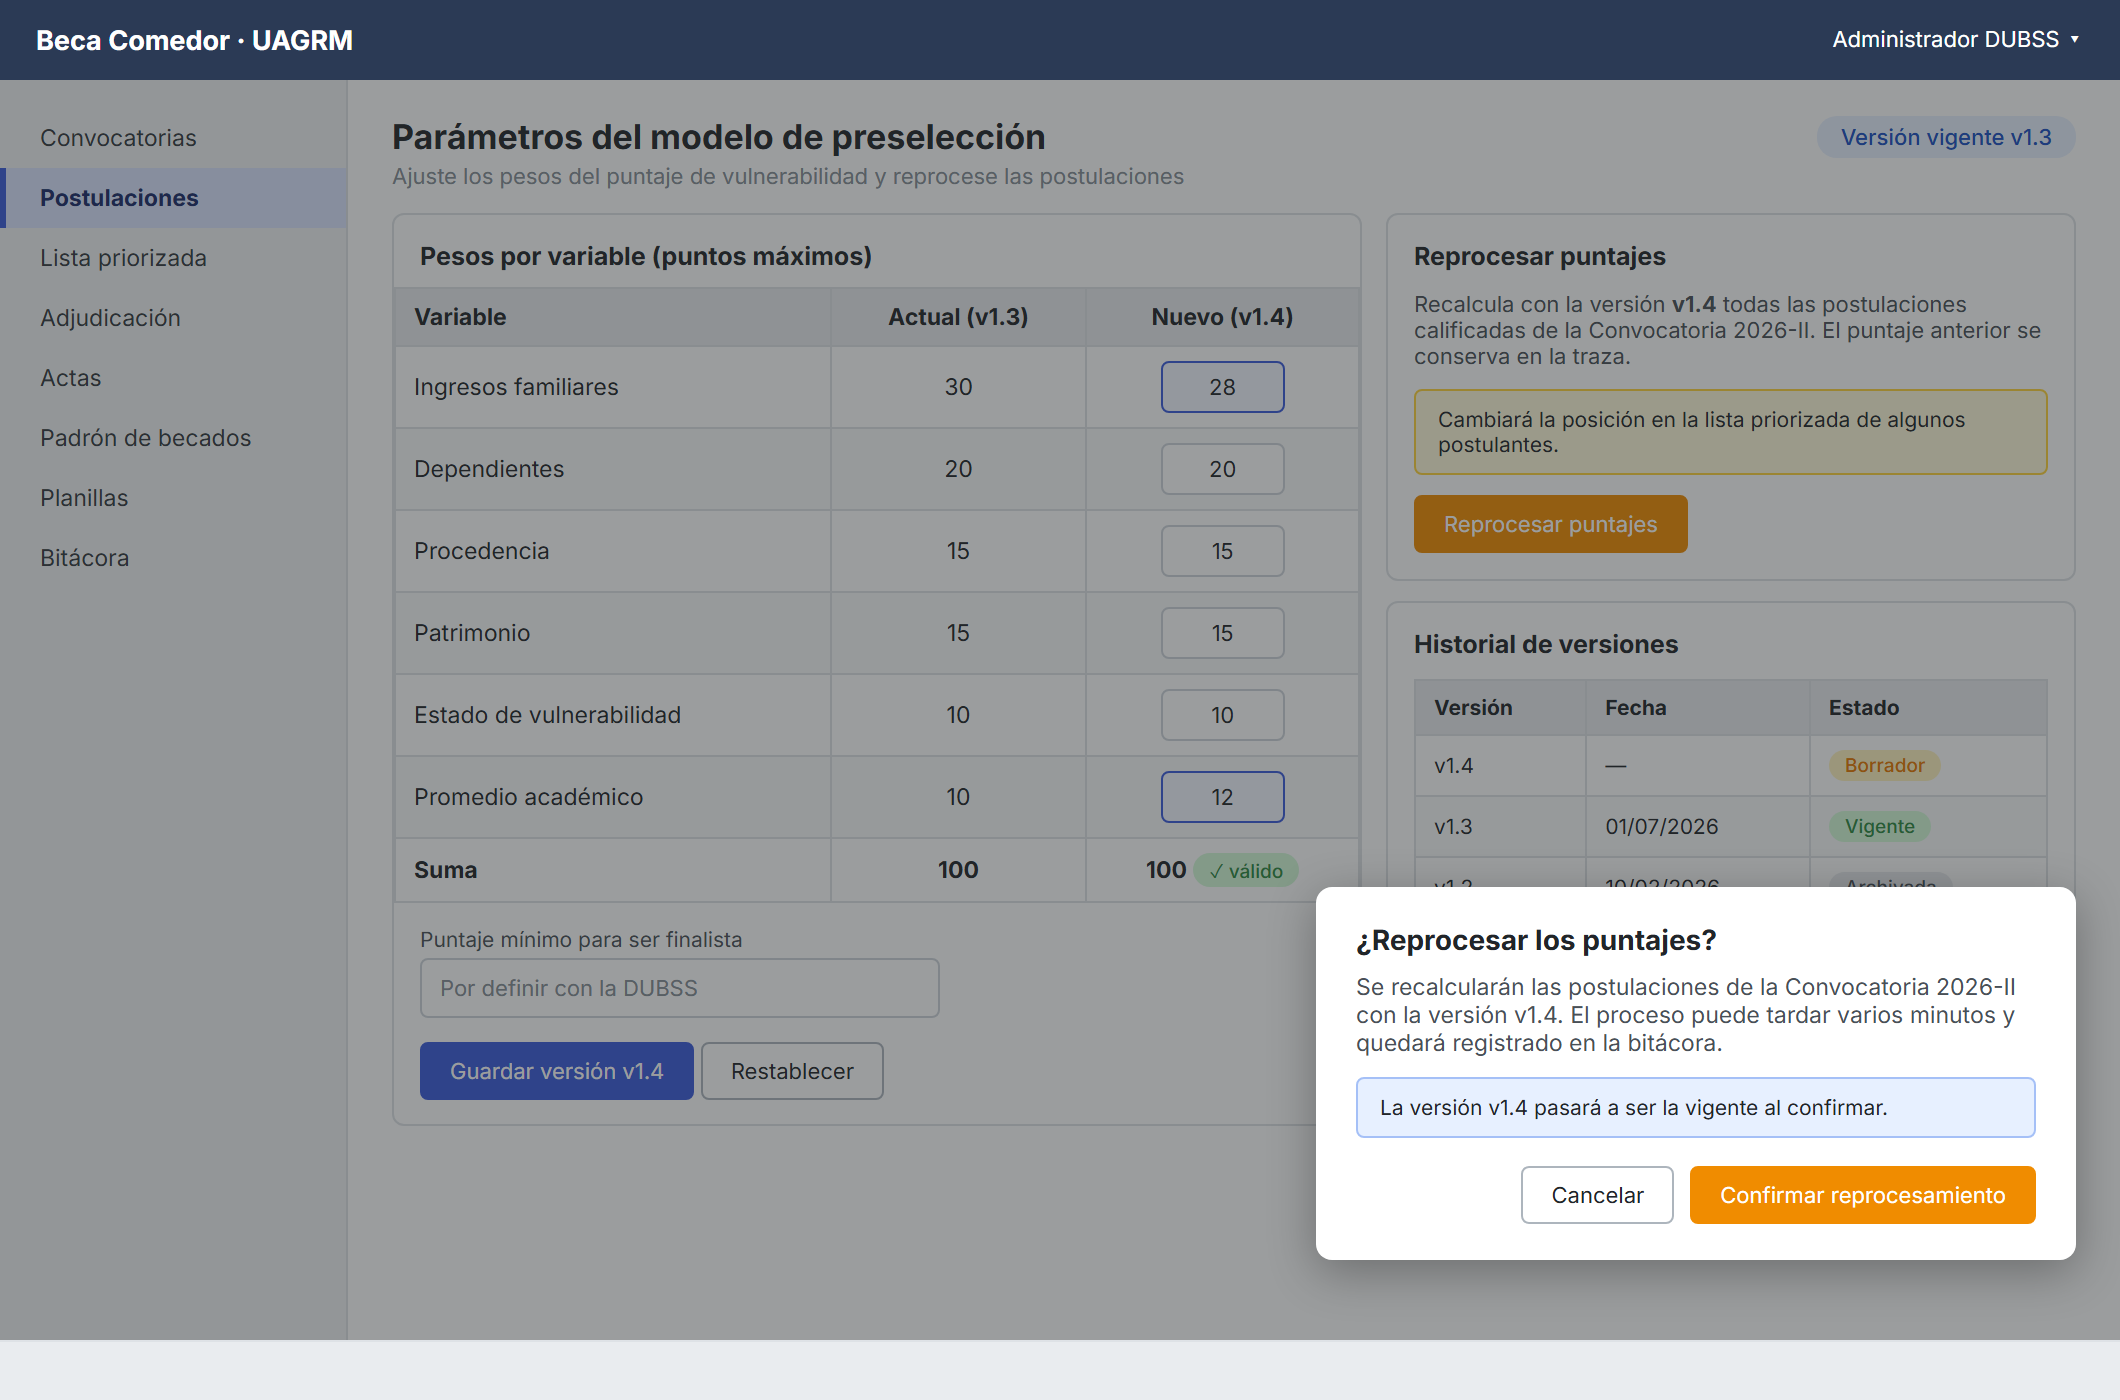
\includegraphics[width=\textwidth,height=0.75\textheight,keepaspectratio]{images/146_Mockup_CU26_Parametrizar_modelo.png}

\smallskip
\noindent\raggedright\textit{Nota.} Elaboración propia.
\end{figure}


